%!TEX root = ../main.tex
% Generado del archivo CSV de Google Forms. Corte: 15/11/2026.
% Insertar desde capitulos/07-resultados.tex mediante %!TEX root = ../main.tex
% Generado del archivo CSV de Google Forms. Corte: 15/11/2026.
% Insertar desde capitulos/07-resultados.tex mediante %!TEX root = ../main.tex
% Generado del archivo CSV de Google Forms. Corte: 15/11/2026.
% Insertar desde capitulos/07-resultados.tex mediante %!TEX root = ../main.tex
% Generado del archivo CSV de Google Forms. Corte: 15/11/2026.
% Insertar desde capitulos/07-resultados.tex mediante \input{capitulos/07-resultados-encuesta}

\section{Resultados de la encuesta exploratoria}
\label{sec:ml-resultados-encuesta}

Con el propósito de explorar las percepciones de los compradores sobre la seguridad en plataformas digitales y el interés por herramientas preventivas, se aplicó un cuestionario de once preguntas cerradas. El corte de resultados analizado comprende \textbf{61 respuestas} registradas entre el \textbf{10 y el 15 de noviembre de 2026}. El instrumento, sus opciones y las condiciones del relevamiento se incluyen en el apéndice~\ref{apx:encuesta}; el procedimiento se describe en la sección~\ref{subsec:ml-encuesta-metodo}.

La encuesta se difundió mediante contactos del autor y constituye un \textbf{relevamiento exploratorio no probabilístico}. Las cifras expresan percepciones e intenciones declaradas del grupo consultado, sin representatividad estadística de la población general ni evidencia directa de eficacia del motor de detección de fraudes. Las preguntas de selección múltiple admitieron varias alternativas; sus porcentajes se calcularon sobre los 61 participantes y pueden sumar más del 100\,\%.

\begin{table}[H]
\centering
\caption{Síntesis de resultados de la encuesta exploratoria (n=61)}
\label{tab:ml-encuesta-principales}
\small
\begin{tabularx}{\textwidth}{L r r}
\toprule
\tb{Indicador declarado} & \tb{Respuestas} & \tb{Porcentaje} \\
\midrule
Encontró alguna publicación sospechosa & 44/61 & 72,1\,\% \\
Desistió de una compra por desconfianza & 47/61 & 77,0\,\% \\
Calificó la utilidad potencial con 4 o 5 (escala de 1 a 5) & 50/61 & 82,0\,\% \\
Consideraría utilizarla de forma frecuente o ante dudas & 58/61 & 95,1\,\% \\
Asignó 4 o 5 de confianza a los mecanismos actuales & 35/61 & 57,4\,\% \\
\bottomrule
\end{tabularx}
\end{table}

\subsection{Experiencia de compra y criterios de evaluación}

El cuestionario contempló tanto participantes que habían comprado durante los últimos doce meses como otros que no lo habían hecho. El uso de cada plataforma, que podía informarse en conjunto con otras, se presenta en la figura~\ref{fig:ml-encuesta-02}. Mercado Libre fue seleccionado por \textbf{52 personas (85,2\,\%)}. En cuanto a los criterios consultados, los más frecuentes fueron la reputación o calificaciones del vendedor (\textbf{50/61}) y las opiniones de compradores anteriores (\textbf{47/61}), tal como muestra la figura~\ref{fig:ml-encuesta-03}.

\subsection{Percepción de riesgo y confianza}

\textbf{44 participantes (72,1\,\%)} señalaron haber encontrado alguna publicación potencialmente sospechosa (figura~\ref{fig:ml-encuesta-04}), mientras que \textbf{47 (77,0\,\%)} indicaron haber desistido de una compra por desconfianza (figura~\ref{fig:ml-encuesta-05}). Ambas preguntas recogen experiencias autopercibidas: no identifican ni verifican casos reales de fraude.

La confianza en los mecanismos actuales de seguridad y reputación se distribuyó en la escala de 1 a 5, con 35 respuestas en los valores 4 o 5 (\textbf{57,4\,\%}). Entre las características que generaron mayor desconfianza se destacaron el precio considerablemente inferior al de ofertas comparables (\textbf{38 respuestas}), la ausencia de calificaciones u opiniones (\textbf{37}) y la solicitud de pago fuera de la plataforma (\textbf{35}). Se trata de percepciones de los participantes y no de una validación de esos indicadores como predictores de fraude.

\subsection{Utilidad percibida e intención declarada de uso}

Tras presentar una descripción conceptual de una herramienta independiente de análisis preventivo, \textbf{50 participantes (82,0\,\%)} asignaron una utilidad de 4 o 5 en una escala de cinco puntos (figura~\ref{fig:ml-encuesta-08}). Además, \textbf{58 (95,1\,\%)} manifestaron que probablemente utilizarían una herramienta gratuita con frecuencia o ante publicaciones que les generaran dudas (figura~\ref{fig:ml-encuesta-09}). Estas respuestas sugieren \emph{interés declarado} y no constituyen evidencia de adopción efectiva.

En cuanto a funcionalidades, la opción más señalada fue la información sobre el historial comercial del vendedor (\textbf{36 respuestas; 59,0\,\%}). Las advertencias sobre datos insuficientes y la explicación de los factores de riesgo reunieron 26 selecciones cada una. Entre las preocupaciones, destacaron la recopilación innecesaria de datos personales (\textbf{33 respuestas}), la información desactualizada (\textbf{30}) y las advertencias incorrectas (\textbf{26}). Estos resultados sirven para orientar prioridades de transparencia, privacidad y calidad de datos, pero por sí solos no validan decisiones técnicas específicas.

\subsection{Alcance y limitaciones del relevamiento}

La distribución del formulario entre contactos y la participación voluntaria introducen posibles \textbf{sesgos de selección y autoselección}. El instrumento no relevó variables sociodemográficas ni verificó en forma independiente las experiencias declaradas. Por consiguiente, no es posible generalizar los resultados a la totalidad de compradores ni estimar márgenes de error de muestreo probabilístico. Asimismo, la descripción conceptual de MarketLens puede influir en las valoraciones de utilidad e intención de uso.

Estas evidencias complementan la justificación del problema abordado y permiten identificar prioridades expresadas por las personas encuestadas. No deben confundirse con pruebas de usabilidad del prototipo, validaciones de precisión del índice de riesgo o una medición de su impacto real en la prevención de estafas. El presente corte corresponde a 61 respuestas; de incorporarse nuevas respuestas, deben recalcularse todos los porcentajes y sustituirse los gráficos correspondientes.

\subsection{Distribución completa de respuestas}

Las figuras siguientes presentan las frecuencias absolutas y los porcentajes observados para las once preguntas, incluida la opción de valoración no seleccionada en las escalas. En preguntas de selección múltiple, el denominador continúa siendo el número total de participantes (61).
\begin{figure}[H]
\centering
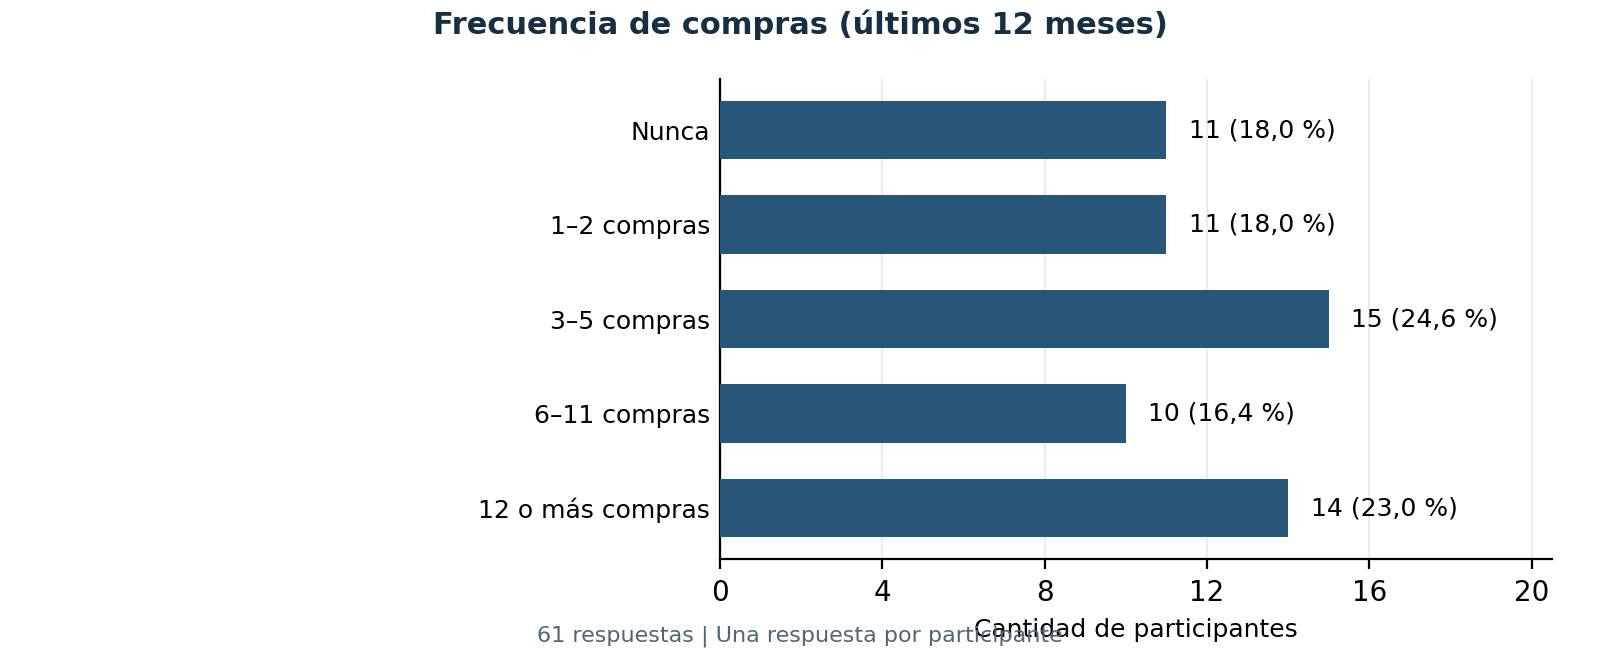
\includegraphics[width=0.94\textwidth,height=0.37\textheight,keepaspectratio]{figuras/marketlens/encuesta/pregunta_01.png}
\caption{Frecuencia de compra declarada en marketplaces durante los últimos doce meses (n=61).}\label{fig:ml-encuesta-01}
\end{figure}

\begin{figure}[H]
\centering
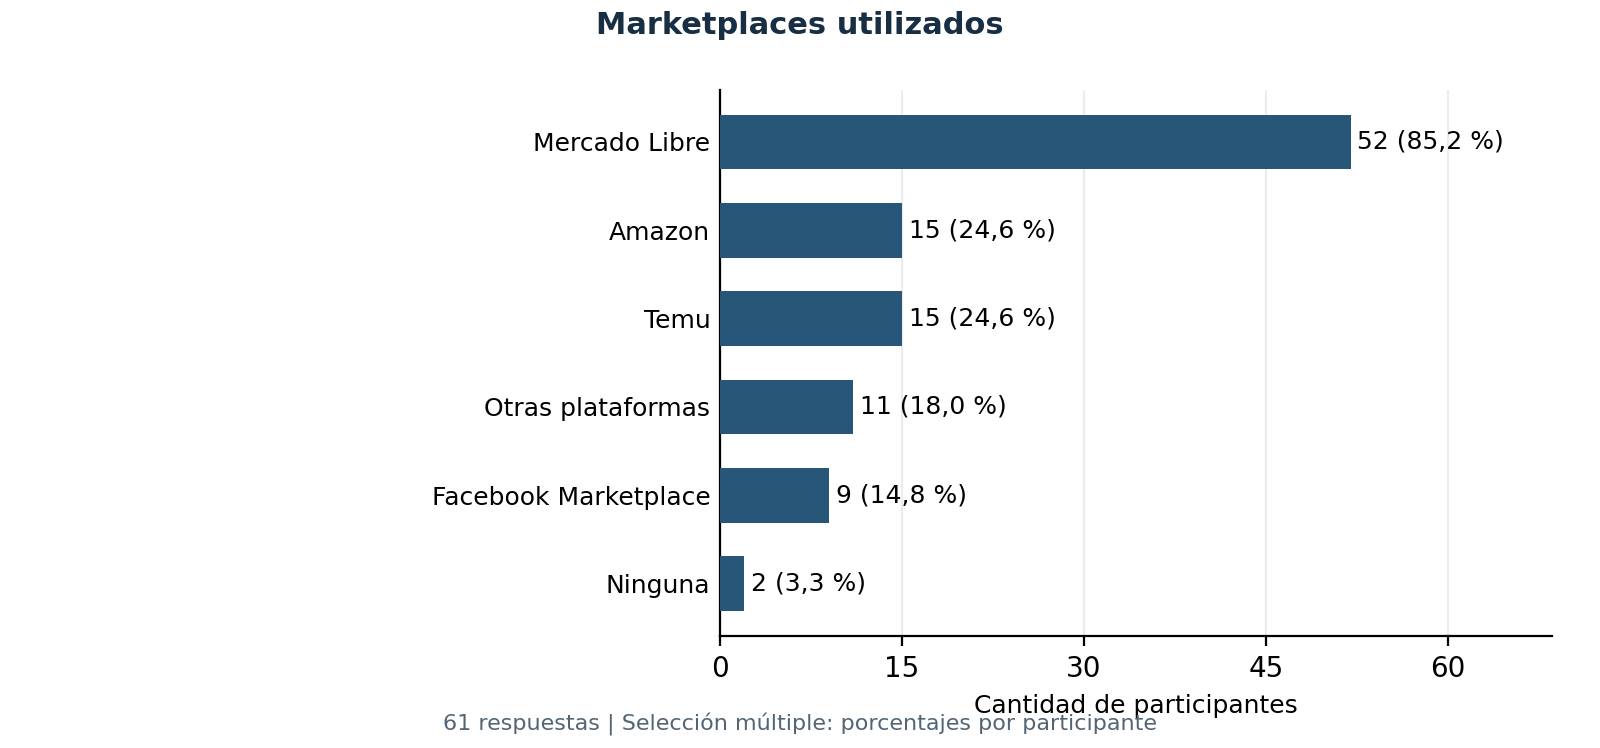
\includegraphics[width=0.94\textwidth,height=0.37\textheight,keepaspectratio]{figuras/marketlens/encuesta/pregunta_02.png}
\caption{Plataformas utilizadas por los encuestados durante los últimos doce meses (n=61).}\label{fig:ml-encuesta-02}
\end{figure}

\begin{figure}[H]
\centering
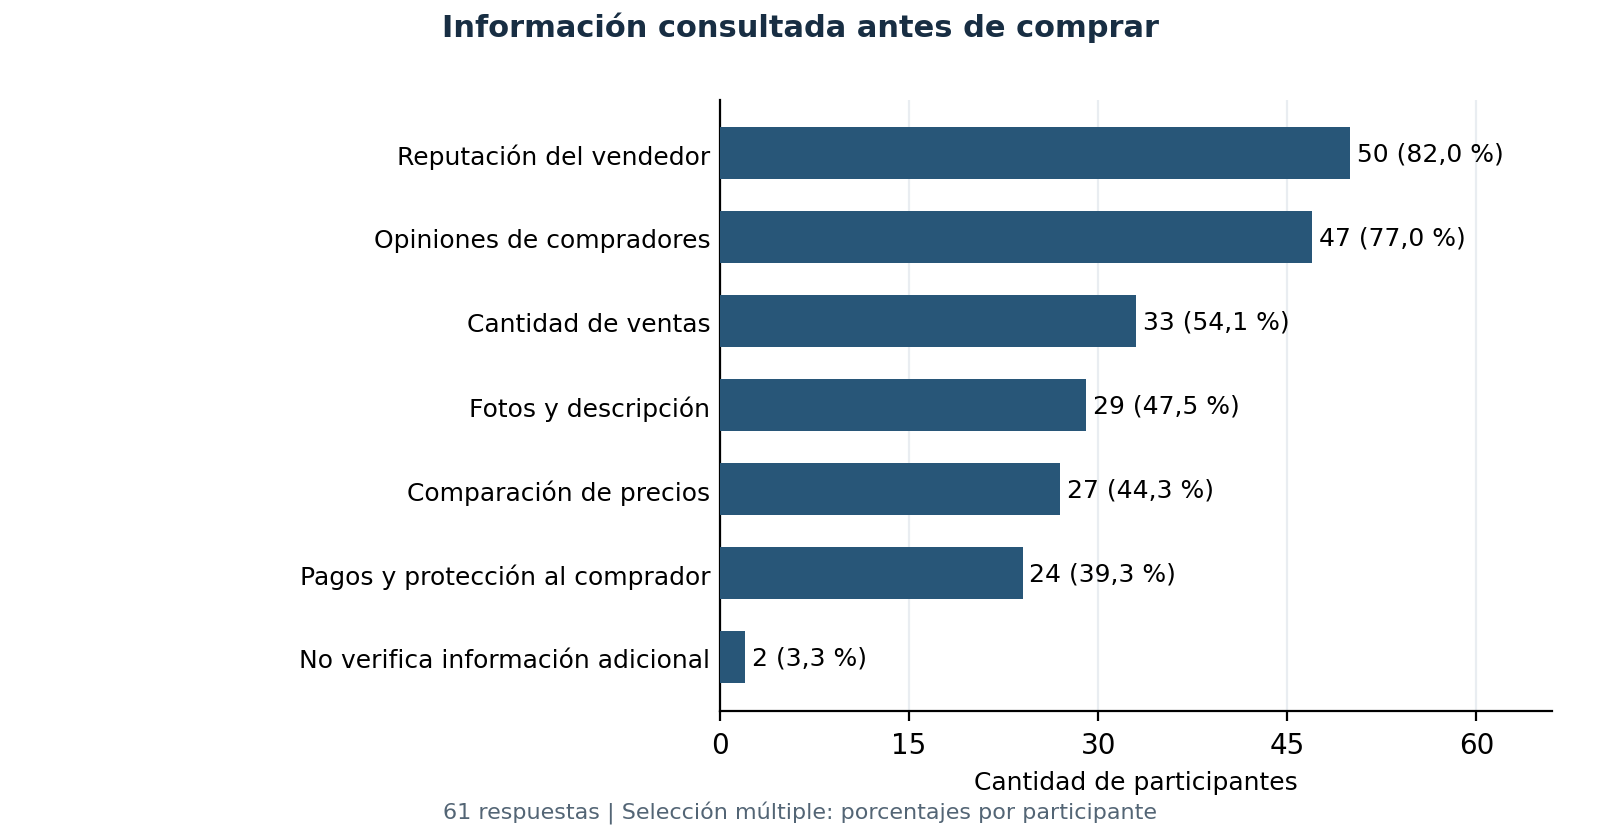
\includegraphics[width=0.94\textwidth,height=0.37\textheight,keepaspectratio]{figuras/marketlens/encuesta/pregunta_03.png}
\caption{Información habitualmente consultada para evaluar publicaciones o vendedores (n=61).}\label{fig:ml-encuesta-03}
\end{figure}

\begin{figure}[H]
\centering
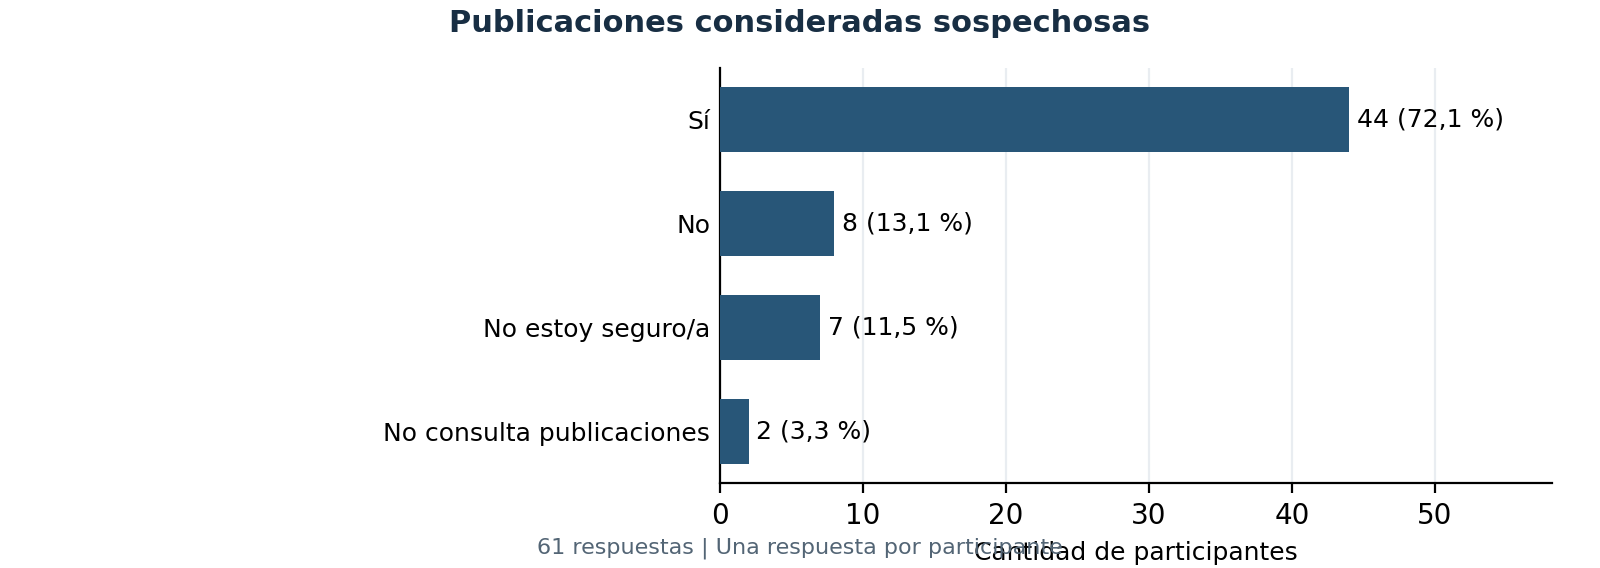
\includegraphics[width=0.94\textwidth,height=0.37\textheight,keepaspectratio]{figuras/marketlens/encuesta/pregunta_04.png}
\caption{Encuestados que identificaron publicaciones potencialmente sospechosas (n=61).}\label{fig:ml-encuesta-04}
\end{figure}

\begin{figure}[H]
\centering
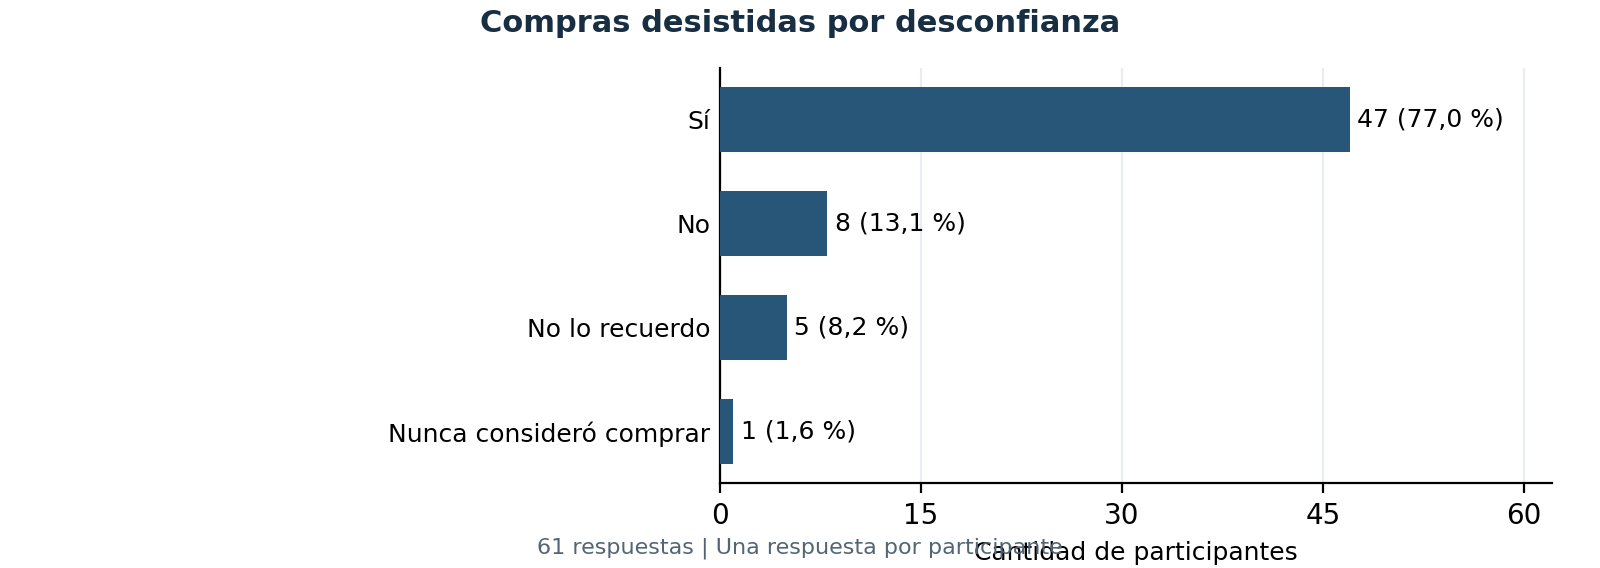
\includegraphics[width=0.94\textwidth,height=0.37\textheight,keepaspectratio]{figuras/marketlens/encuesta/pregunta_05.png}
\caption{Encuestados que desistieron de una compra por desconfianza (n=61).}\label{fig:ml-encuesta-05}
\end{figure}

\begin{figure}[H]
\centering
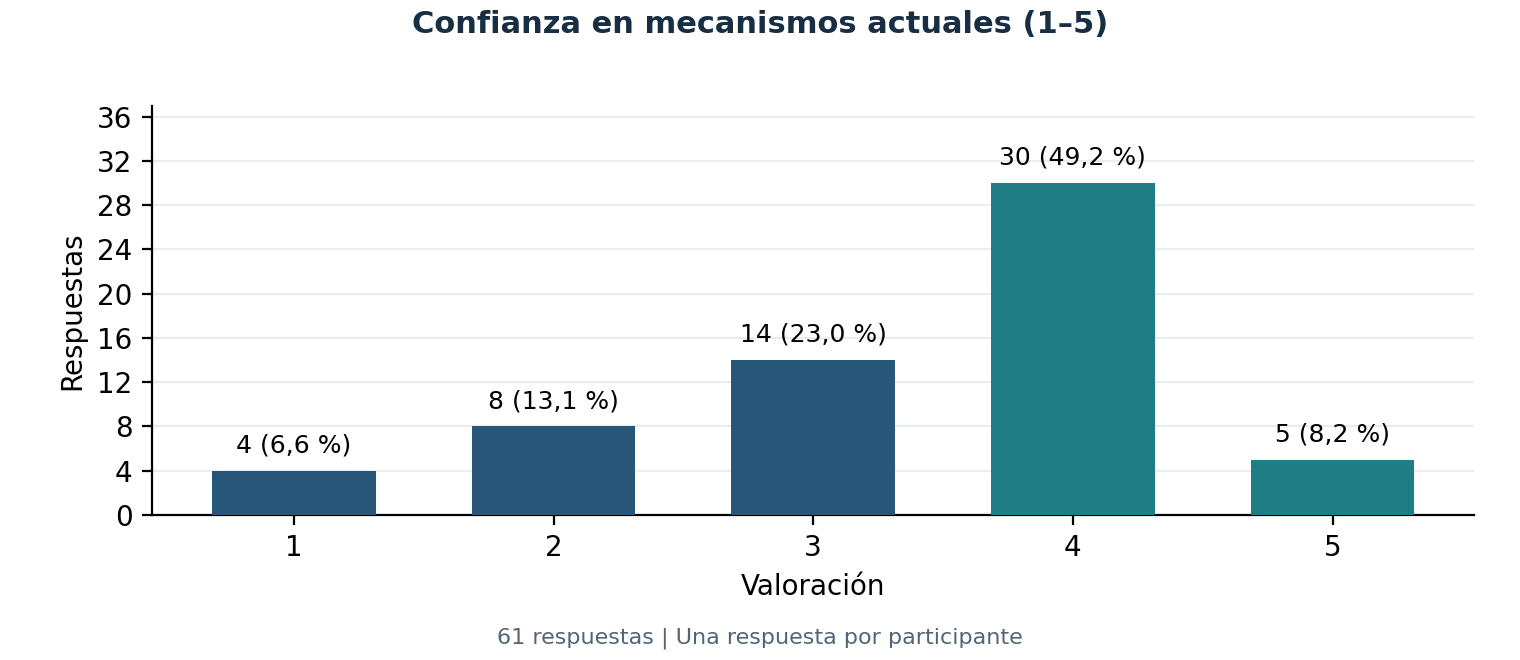
\includegraphics[width=0.94\textwidth,height=0.37\textheight,keepaspectratio]{figuras/marketlens/encuesta/pregunta_06.png}
\caption{Confianza declarada en los mecanismos actuales de seguridad y reputación (n=61).}\label{fig:ml-encuesta-06}
\end{figure}

\begin{figure}[H]
\centering
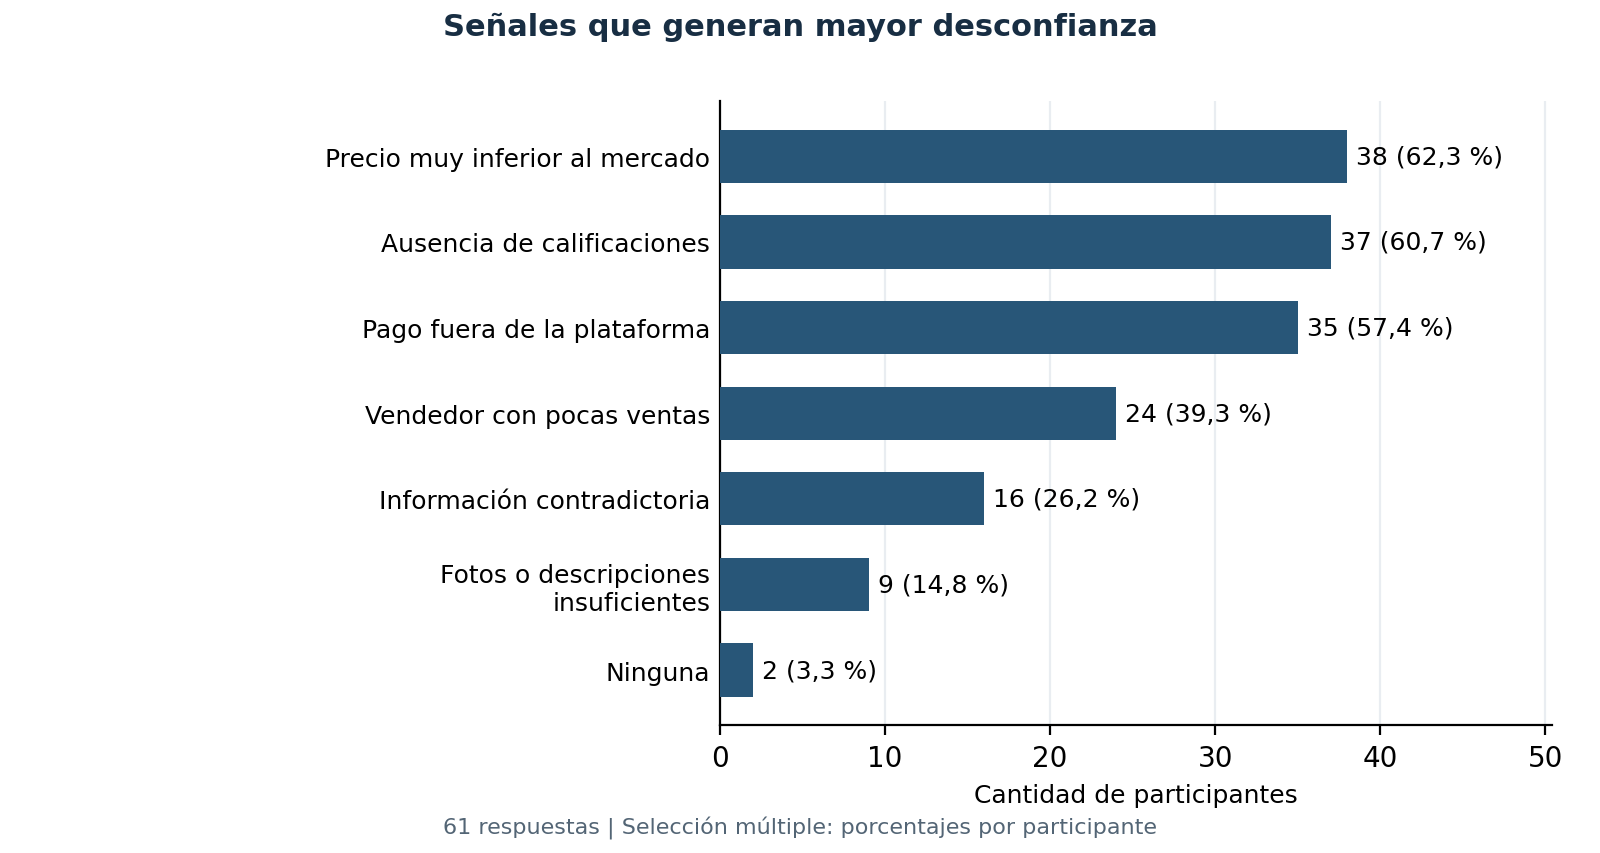
\includegraphics[width=0.94\textwidth,height=0.37\textheight,keepaspectratio]{figuras/marketlens/encuesta/pregunta_07.png}
\caption{Características de publicaciones que generan mayor desconfianza (n=61).}\label{fig:ml-encuesta-07}
\end{figure}

\begin{figure}[H]
\centering
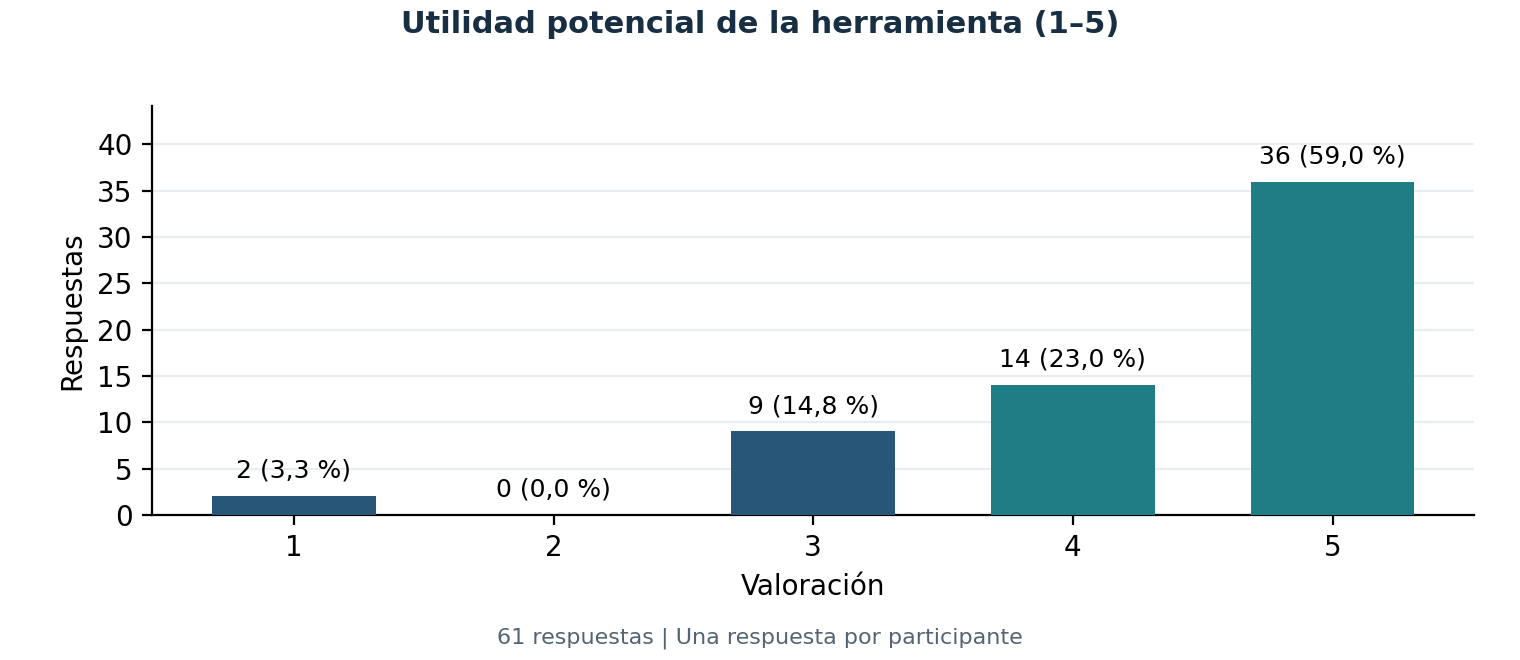
\includegraphics[width=0.94\textwidth,height=0.37\textheight,keepaspectratio]{figuras/marketlens/encuesta/pregunta_08.png}
\caption{Utilidad potencial atribuida a una herramienta de análisis preventivo (n=61).}\label{fig:ml-encuesta-08}
\end{figure}

\begin{figure}[H]
\centering
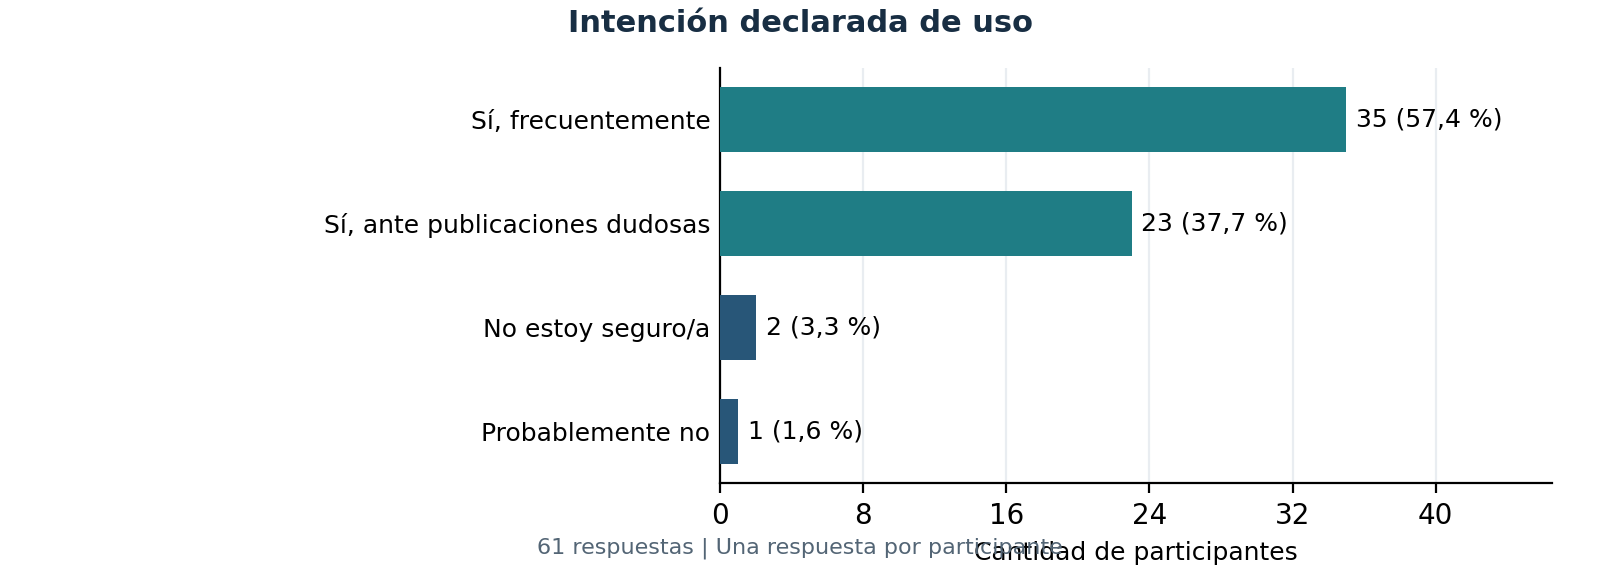
\includegraphics[width=0.94\textwidth,height=0.37\textheight,keepaspectratio]{figuras/marketlens/encuesta/pregunta_09.png}
\caption{Intención declarada de utilización de una herramienta gratuita como la propuesta (n=61).}\label{fig:ml-encuesta-09}
\end{figure}

\begin{figure}[H]
\centering
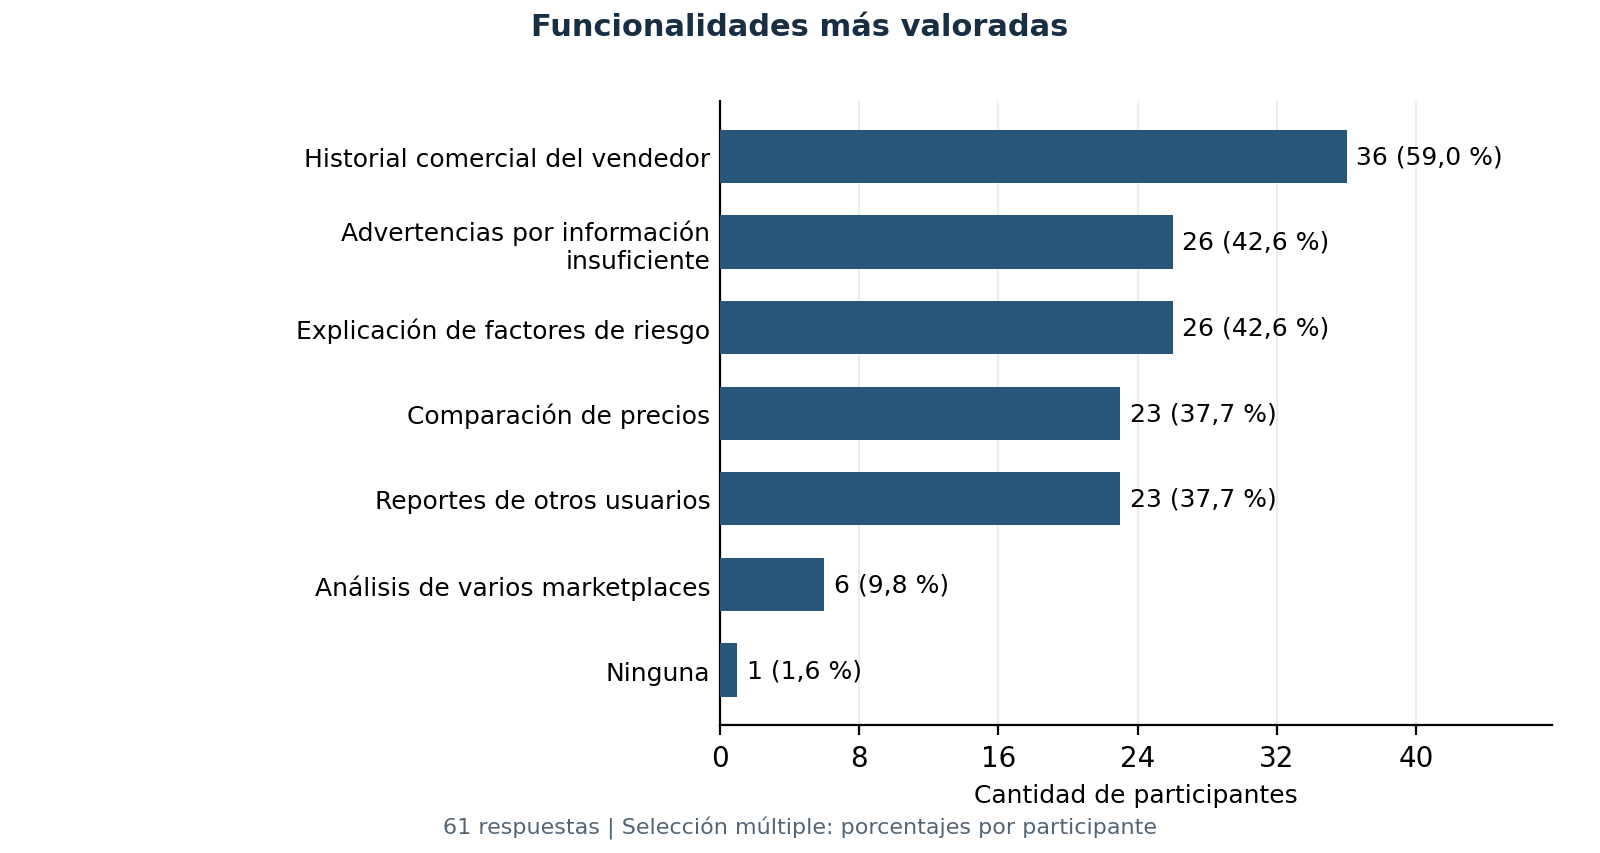
\includegraphics[width=0.94\textwidth,height=0.37\textheight,keepaspectratio]{figuras/marketlens/encuesta/pregunta_10.png}
\caption{Funcionalidades prioritarias para una herramienta de análisis preventivo (n=61).}\label{fig:ml-encuesta-10}
\end{figure}

\begin{figure}[H]
\centering
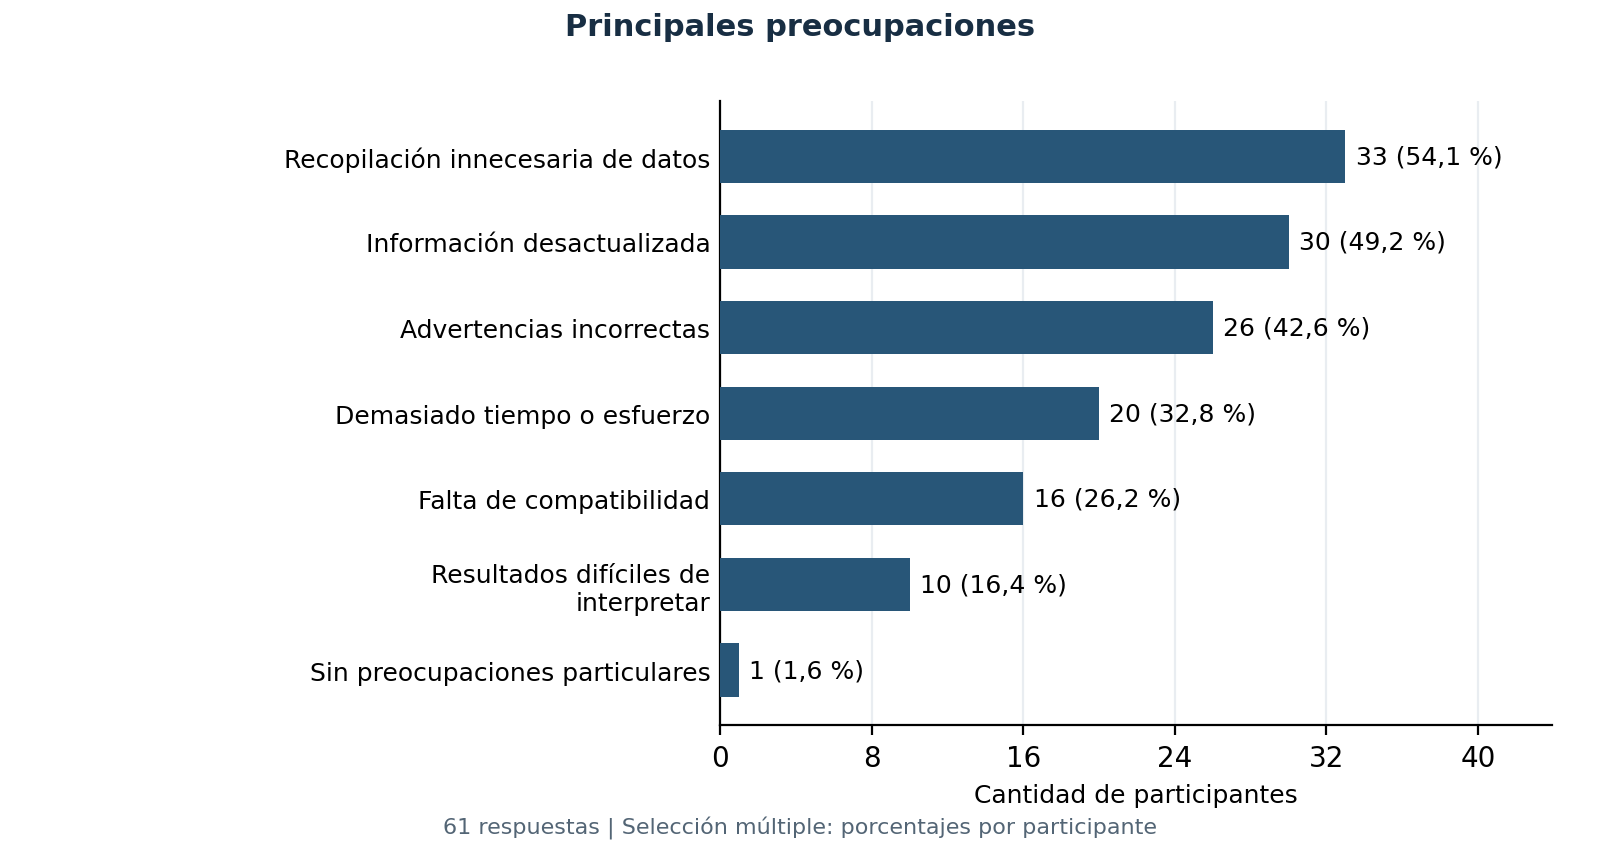
\includegraphics[width=0.94\textwidth,height=0.37\textheight,keepaspectratio]{figuras/marketlens/encuesta/pregunta_11.png}
\caption{Principales preocupaciones respecto del uso de la herramienta (n=61).}\label{fig:ml-encuesta-11}
\end{figure}



\section{Resultados de la encuesta exploratoria}
\label{sec:ml-resultados-encuesta}

Con el propósito de explorar las percepciones de los compradores sobre la seguridad en plataformas digitales y el interés por herramientas preventivas, se aplicó un cuestionario de once preguntas cerradas. El corte de resultados analizado comprende \textbf{61 respuestas} registradas entre el \textbf{10 y el 15 de noviembre de 2026}. El instrumento, sus opciones y las condiciones del relevamiento se incluyen en el apéndice~\ref{apx:encuesta}; el procedimiento se describe en la sección~\ref{subsec:ml-encuesta-metodo}.

La encuesta se difundió mediante contactos del autor y constituye un \textbf{relevamiento exploratorio no probabilístico}. Las cifras expresan percepciones e intenciones declaradas del grupo consultado, sin representatividad estadística de la población general ni evidencia directa de eficacia del motor de detección de fraudes. Las preguntas de selección múltiple admitieron varias alternativas; sus porcentajes se calcularon sobre los 61 participantes y pueden sumar más del 100\,\%.

\begin{table}[H]
\centering
\caption{Síntesis de resultados de la encuesta exploratoria (n=61)}
\label{tab:ml-encuesta-principales}
\small
\begin{tabularx}{\textwidth}{L r r}
\toprule
\tb{Indicador declarado} & \tb{Respuestas} & \tb{Porcentaje} \\
\midrule
Encontró alguna publicación sospechosa & 44/61 & 72,1\,\% \\
Desistió de una compra por desconfianza & 47/61 & 77,0\,\% \\
Calificó la utilidad potencial con 4 o 5 (escala de 1 a 5) & 50/61 & 82,0\,\% \\
Consideraría utilizarla de forma frecuente o ante dudas & 58/61 & 95,1\,\% \\
Asignó 4 o 5 de confianza a los mecanismos actuales & 35/61 & 57,4\,\% \\
\bottomrule
\end{tabularx}
\end{table}

\subsection{Experiencia de compra y criterios de evaluación}

El cuestionario contempló tanto participantes que habían comprado durante los últimos doce meses como otros que no lo habían hecho. El uso de cada plataforma, que podía informarse en conjunto con otras, se presenta en la figura~\ref{fig:ml-encuesta-02}. Mercado Libre fue seleccionado por \textbf{52 personas (85,2\,\%)}. En cuanto a los criterios consultados, los más frecuentes fueron la reputación o calificaciones del vendedor (\textbf{50/61}) y las opiniones de compradores anteriores (\textbf{47/61}), tal como muestra la figura~\ref{fig:ml-encuesta-03}.

\subsection{Percepción de riesgo y confianza}

\textbf{44 participantes (72,1\,\%)} señalaron haber encontrado alguna publicación potencialmente sospechosa (figura~\ref{fig:ml-encuesta-04}), mientras que \textbf{47 (77,0\,\%)} indicaron haber desistido de una compra por desconfianza (figura~\ref{fig:ml-encuesta-05}). Ambas preguntas recogen experiencias autopercibidas: no identifican ni verifican casos reales de fraude.

La confianza en los mecanismos actuales de seguridad y reputación se distribuyó en la escala de 1 a 5, con 35 respuestas en los valores 4 o 5 (\textbf{57,4\,\%}). Entre las características que generaron mayor desconfianza se destacaron el precio considerablemente inferior al de ofertas comparables (\textbf{38 respuestas}), la ausencia de calificaciones u opiniones (\textbf{37}) y la solicitud de pago fuera de la plataforma (\textbf{35}). Se trata de percepciones de los participantes y no de una validación de esos indicadores como predictores de fraude.

\subsection{Utilidad percibida e intención declarada de uso}

Tras presentar una descripción conceptual de una herramienta independiente de análisis preventivo, \textbf{50 participantes (82,0\,\%)} asignaron una utilidad de 4 o 5 en una escala de cinco puntos (figura~\ref{fig:ml-encuesta-08}). Además, \textbf{58 (95,1\,\%)} manifestaron que probablemente utilizarían una herramienta gratuita con frecuencia o ante publicaciones que les generaran dudas (figura~\ref{fig:ml-encuesta-09}). Estas respuestas sugieren \emph{interés declarado} y no constituyen evidencia de adopción efectiva.

En cuanto a funcionalidades, la opción más señalada fue la información sobre el historial comercial del vendedor (\textbf{36 respuestas; 59,0\,\%}). Las advertencias sobre datos insuficientes y la explicación de los factores de riesgo reunieron 26 selecciones cada una. Entre las preocupaciones, destacaron la recopilación innecesaria de datos personales (\textbf{33 respuestas}), la información desactualizada (\textbf{30}) y las advertencias incorrectas (\textbf{26}). Estos resultados sirven para orientar prioridades de transparencia, privacidad y calidad de datos, pero por sí solos no validan decisiones técnicas específicas.

\subsection{Alcance y limitaciones del relevamiento}

La distribución del formulario entre contactos y la participación voluntaria introducen posibles \textbf{sesgos de selección y autoselección}. El instrumento no relevó variables sociodemográficas ni verificó en forma independiente las experiencias declaradas. Por consiguiente, no es posible generalizar los resultados a la totalidad de compradores ni estimar márgenes de error de muestreo probabilístico. Asimismo, la descripción conceptual de MarketLens puede influir en las valoraciones de utilidad e intención de uso.

Estas evidencias complementan la justificación del problema abordado y permiten identificar prioridades expresadas por las personas encuestadas. No deben confundirse con pruebas de usabilidad del prototipo, validaciones de precisión del índice de riesgo o una medición de su impacto real en la prevención de estafas. El presente corte corresponde a 61 respuestas; de incorporarse nuevas respuestas, deben recalcularse todos los porcentajes y sustituirse los gráficos correspondientes.

\subsection{Distribución completa de respuestas}

Las figuras siguientes presentan las frecuencias absolutas y los porcentajes observados para las once preguntas, incluida la opción de valoración no seleccionada en las escalas. En preguntas de selección múltiple, el denominador continúa siendo el número total de participantes (61).
\begin{figure}[H]
\centering
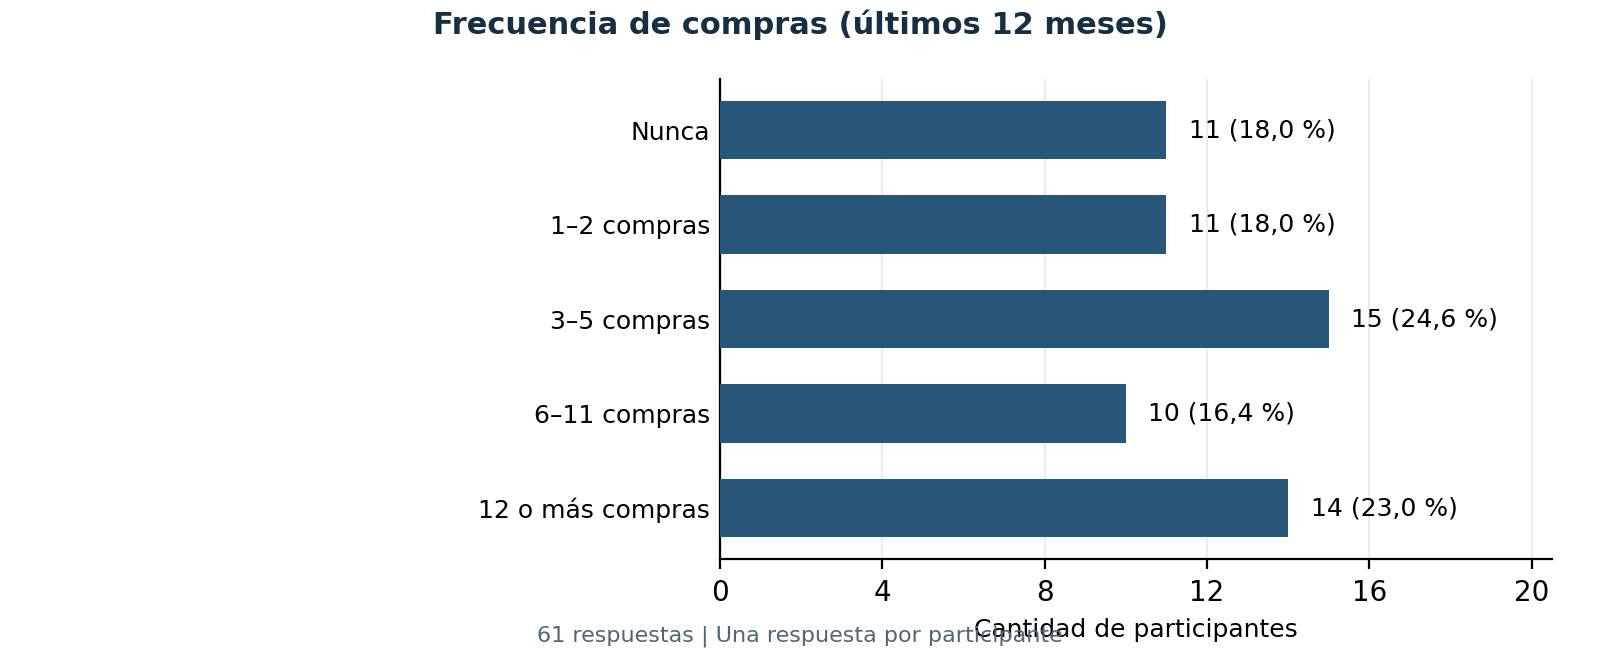
\includegraphics[width=0.94\textwidth,height=0.37\textheight,keepaspectratio]{figuras/marketlens/encuesta/pregunta_01.png}
\caption{Frecuencia de compra declarada en marketplaces durante los últimos doce meses (n=61).}\label{fig:ml-encuesta-01}
\end{figure}

\begin{figure}[H]
\centering
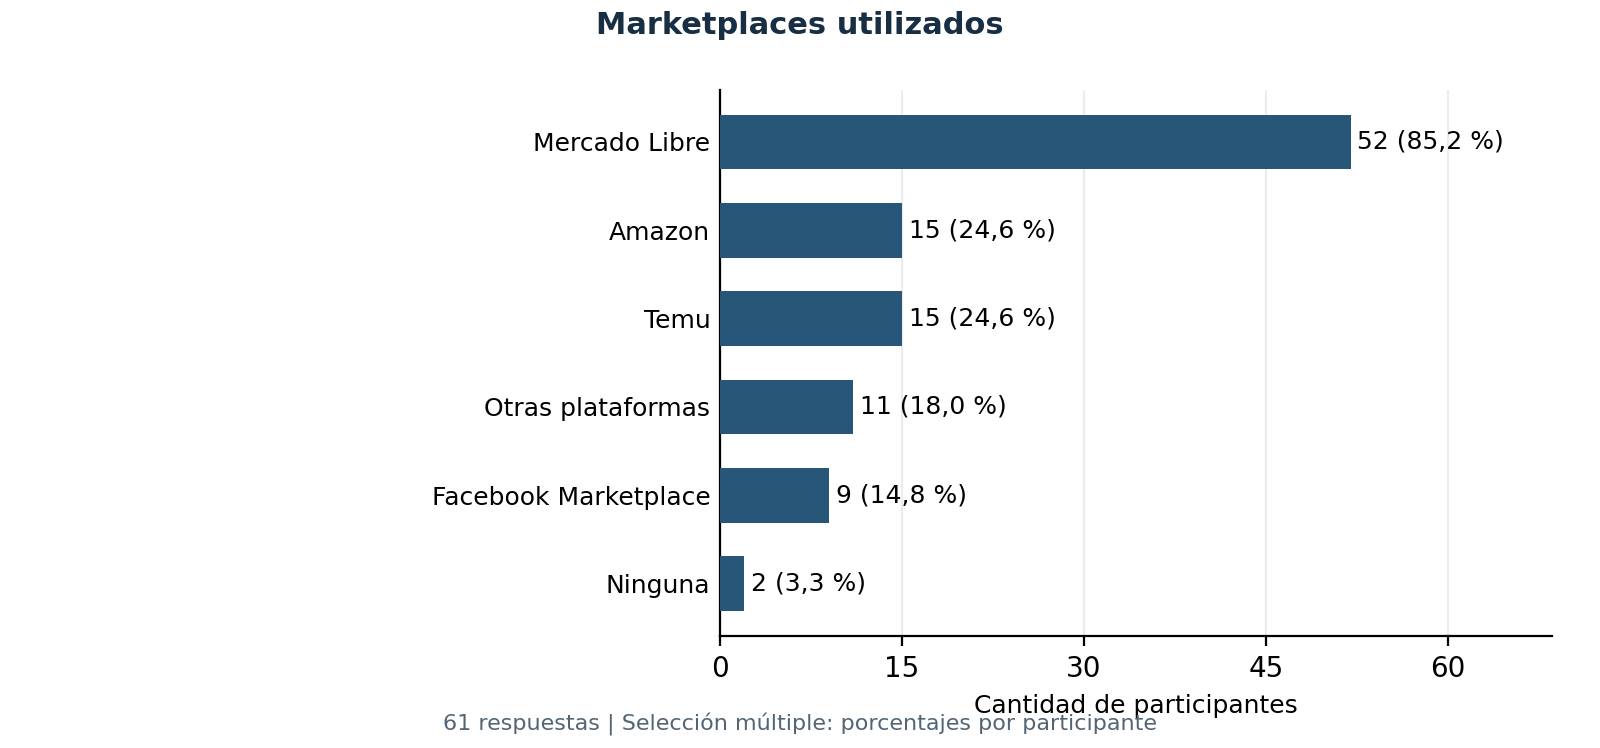
\includegraphics[width=0.94\textwidth,height=0.37\textheight,keepaspectratio]{figuras/marketlens/encuesta/pregunta_02.png}
\caption{Plataformas utilizadas por los encuestados durante los últimos doce meses (n=61).}\label{fig:ml-encuesta-02}
\end{figure}

\begin{figure}[H]
\centering
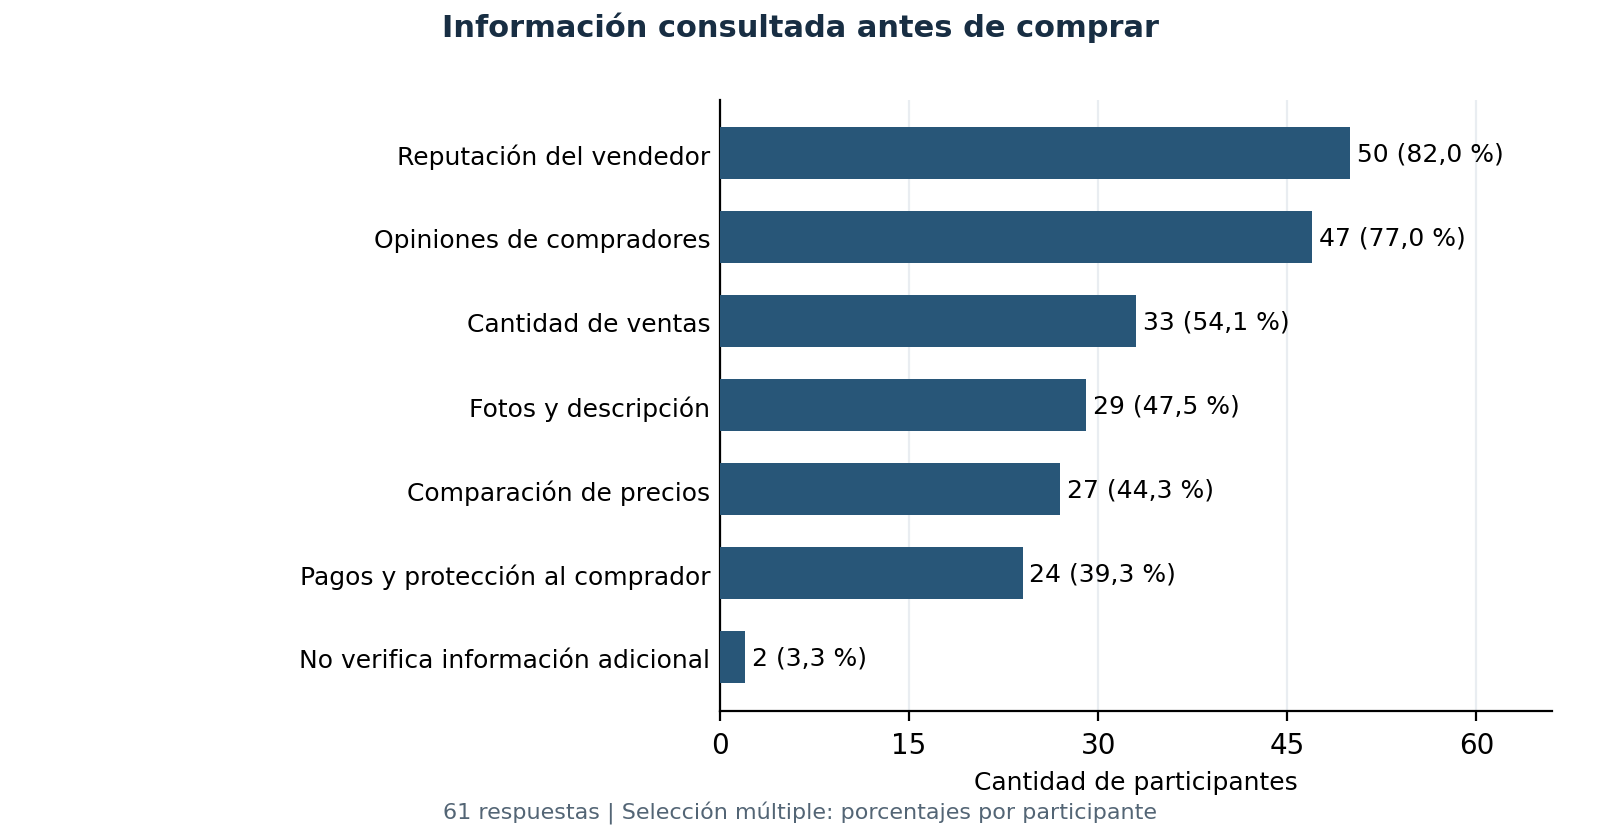
\includegraphics[width=0.94\textwidth,height=0.37\textheight,keepaspectratio]{figuras/marketlens/encuesta/pregunta_03.png}
\caption{Información habitualmente consultada para evaluar publicaciones o vendedores (n=61).}\label{fig:ml-encuesta-03}
\end{figure}

\begin{figure}[H]
\centering
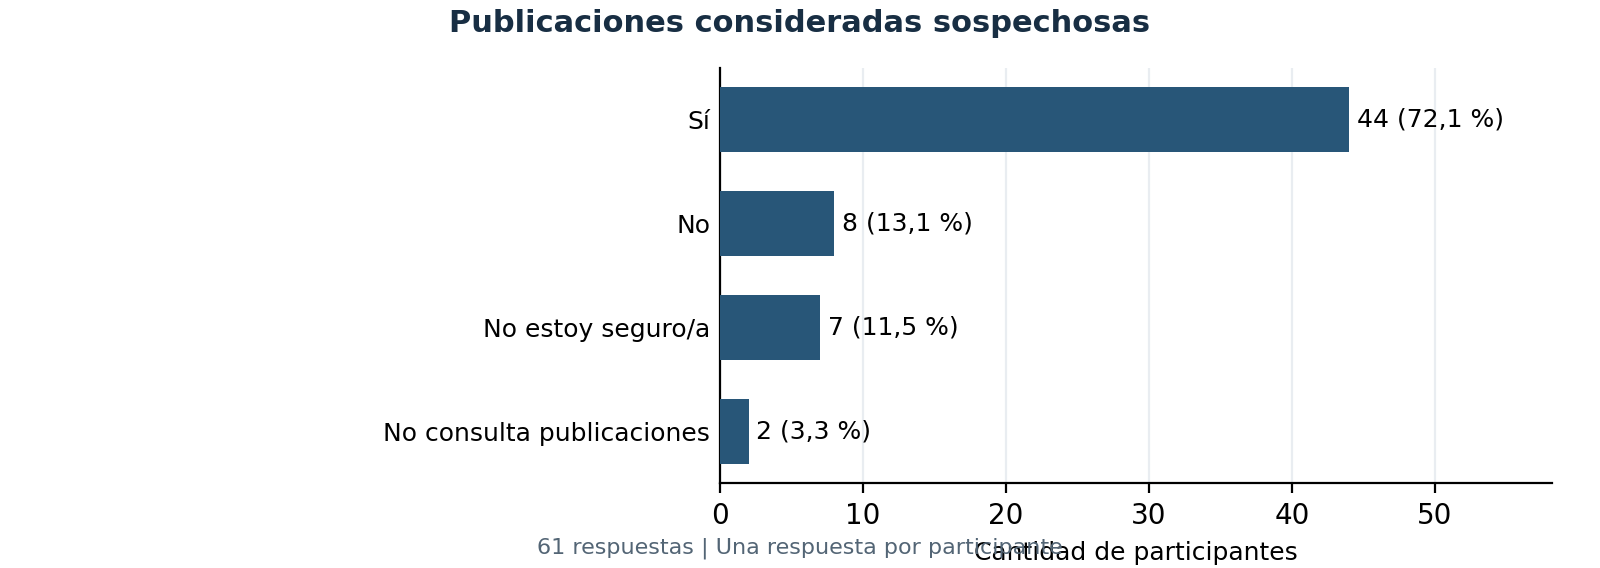
\includegraphics[width=0.94\textwidth,height=0.37\textheight,keepaspectratio]{figuras/marketlens/encuesta/pregunta_04.png}
\caption{Encuestados que identificaron publicaciones potencialmente sospechosas (n=61).}\label{fig:ml-encuesta-04}
\end{figure}

\begin{figure}[H]
\centering
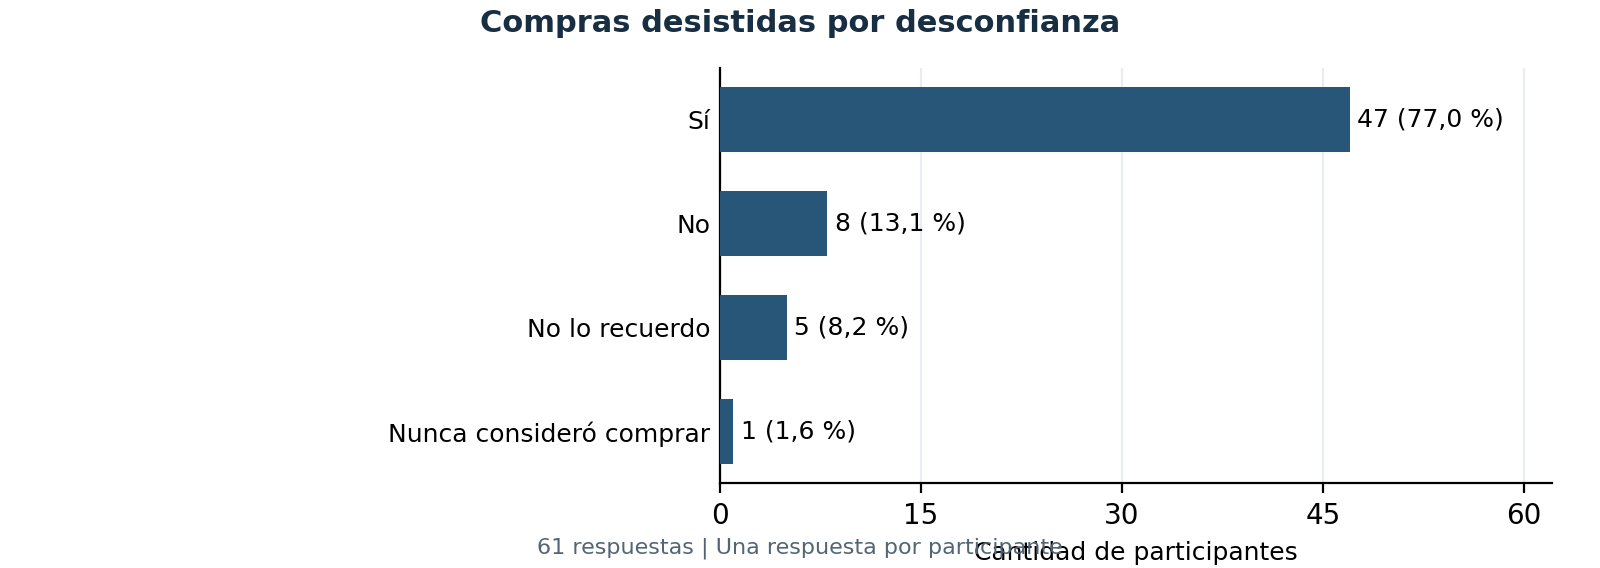
\includegraphics[width=0.94\textwidth,height=0.37\textheight,keepaspectratio]{figuras/marketlens/encuesta/pregunta_05.png}
\caption{Encuestados que desistieron de una compra por desconfianza (n=61).}\label{fig:ml-encuesta-05}
\end{figure}

\begin{figure}[H]
\centering
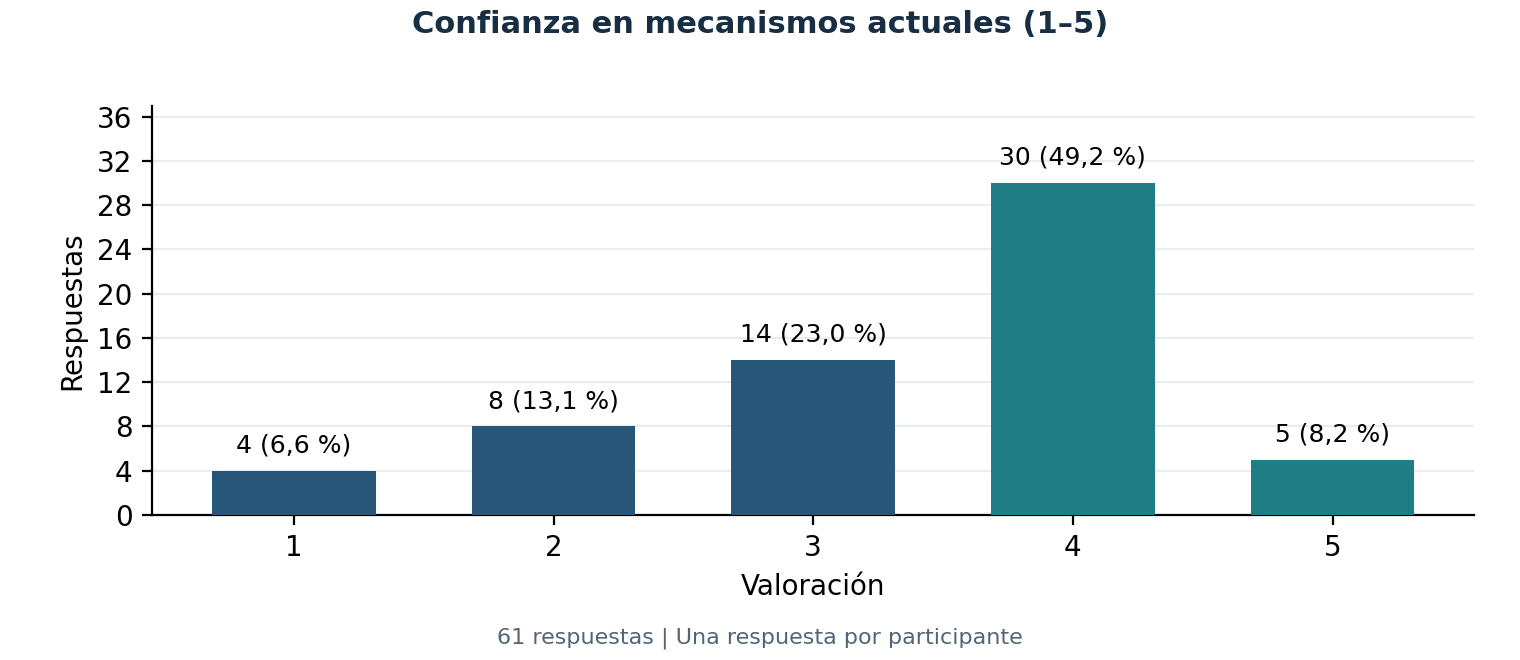
\includegraphics[width=0.94\textwidth,height=0.37\textheight,keepaspectratio]{figuras/marketlens/encuesta/pregunta_06.png}
\caption{Confianza declarada en los mecanismos actuales de seguridad y reputación (n=61).}\label{fig:ml-encuesta-06}
\end{figure}

\begin{figure}[H]
\centering
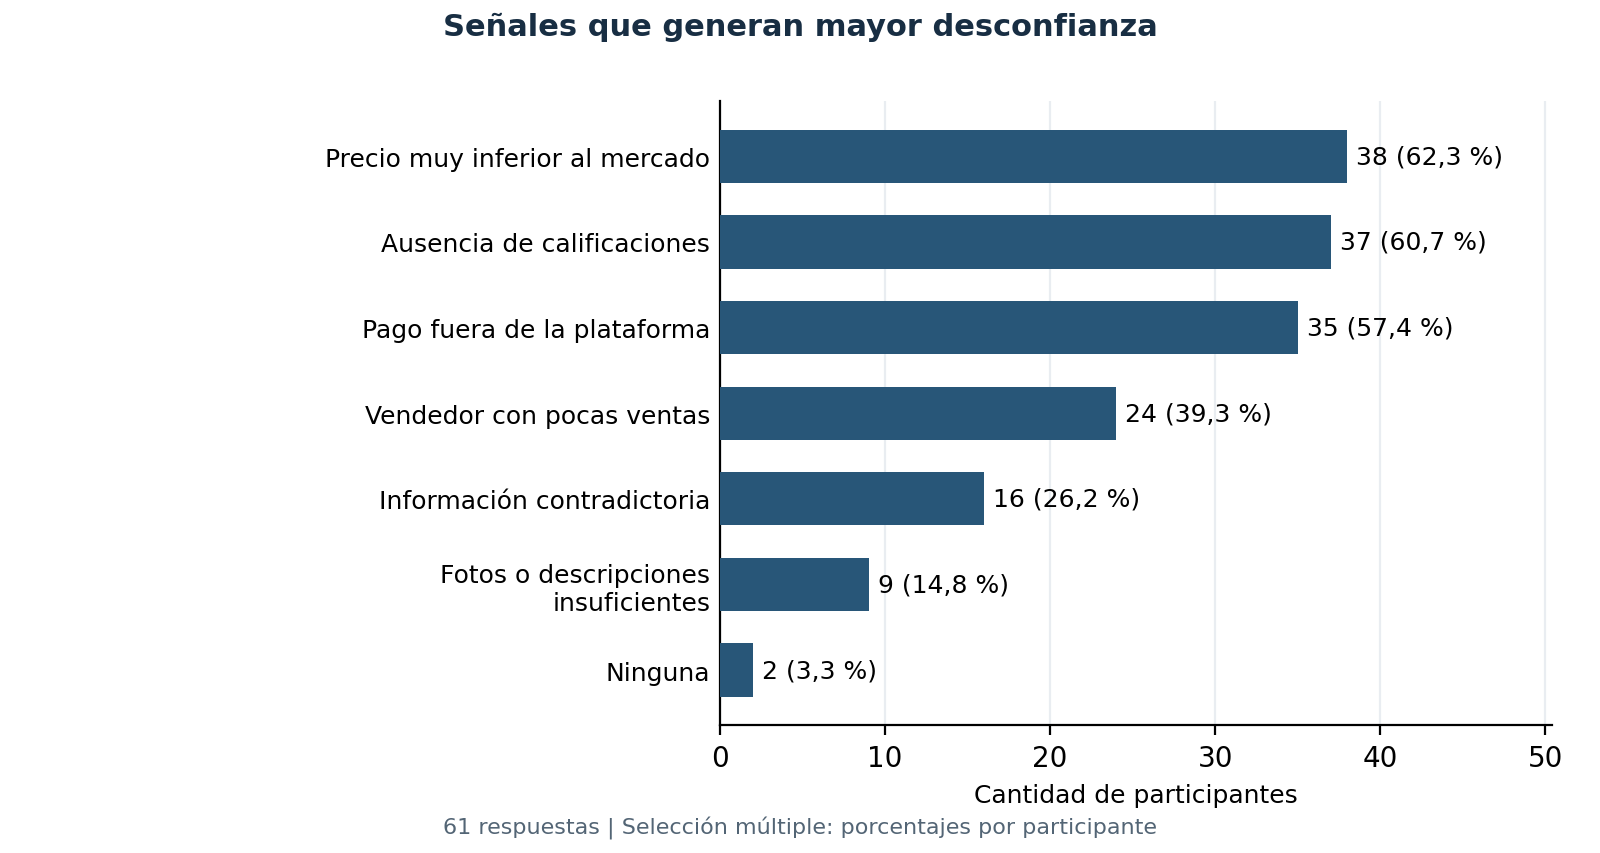
\includegraphics[width=0.94\textwidth,height=0.37\textheight,keepaspectratio]{figuras/marketlens/encuesta/pregunta_07.png}
\caption{Características de publicaciones que generan mayor desconfianza (n=61).}\label{fig:ml-encuesta-07}
\end{figure}

\begin{figure}[H]
\centering
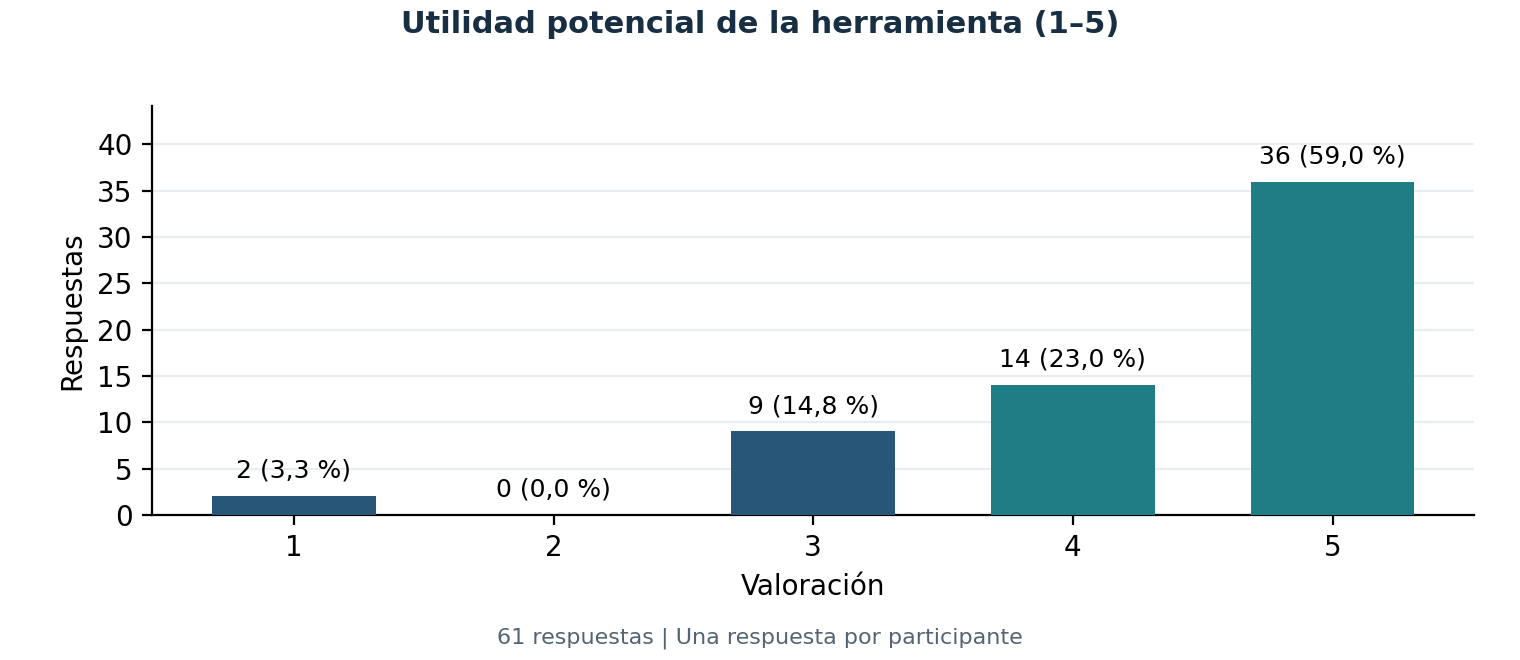
\includegraphics[width=0.94\textwidth,height=0.37\textheight,keepaspectratio]{figuras/marketlens/encuesta/pregunta_08.png}
\caption{Utilidad potencial atribuida a una herramienta de análisis preventivo (n=61).}\label{fig:ml-encuesta-08}
\end{figure}

\begin{figure}[H]
\centering
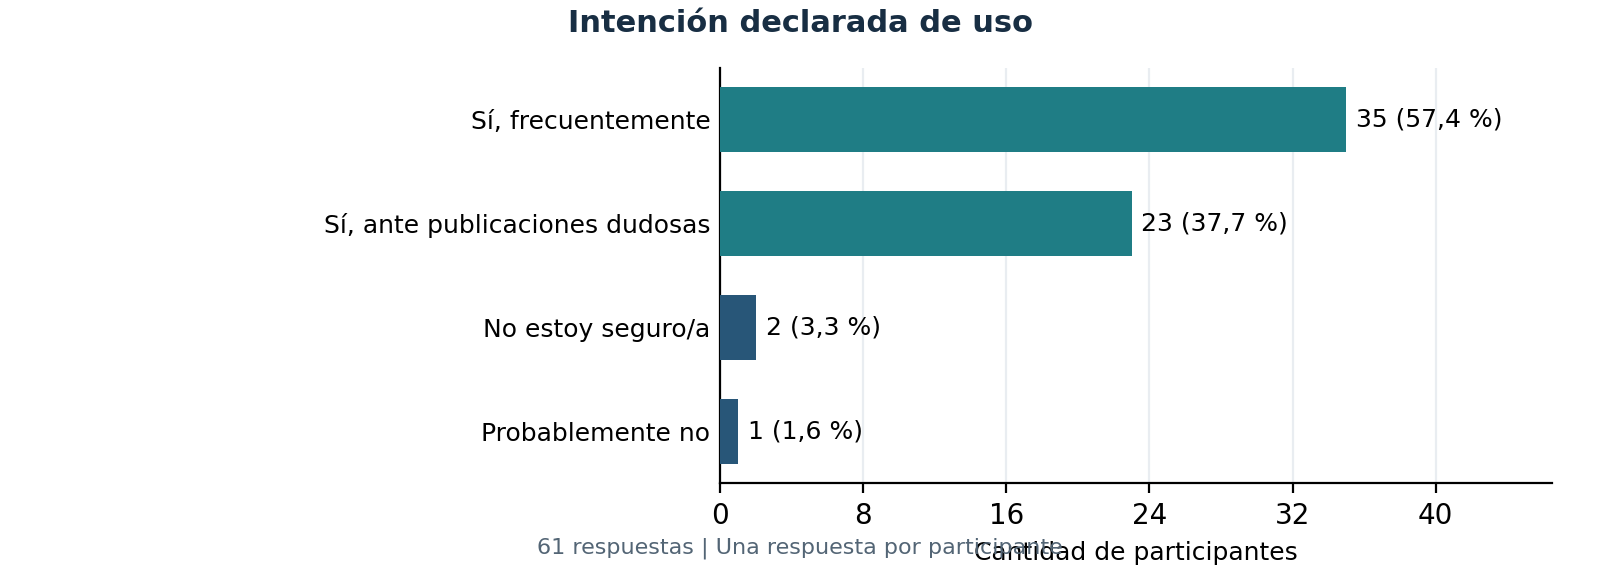
\includegraphics[width=0.94\textwidth,height=0.37\textheight,keepaspectratio]{figuras/marketlens/encuesta/pregunta_09.png}
\caption{Intención declarada de utilización de una herramienta gratuita como la propuesta (n=61).}\label{fig:ml-encuesta-09}
\end{figure}

\begin{figure}[H]
\centering
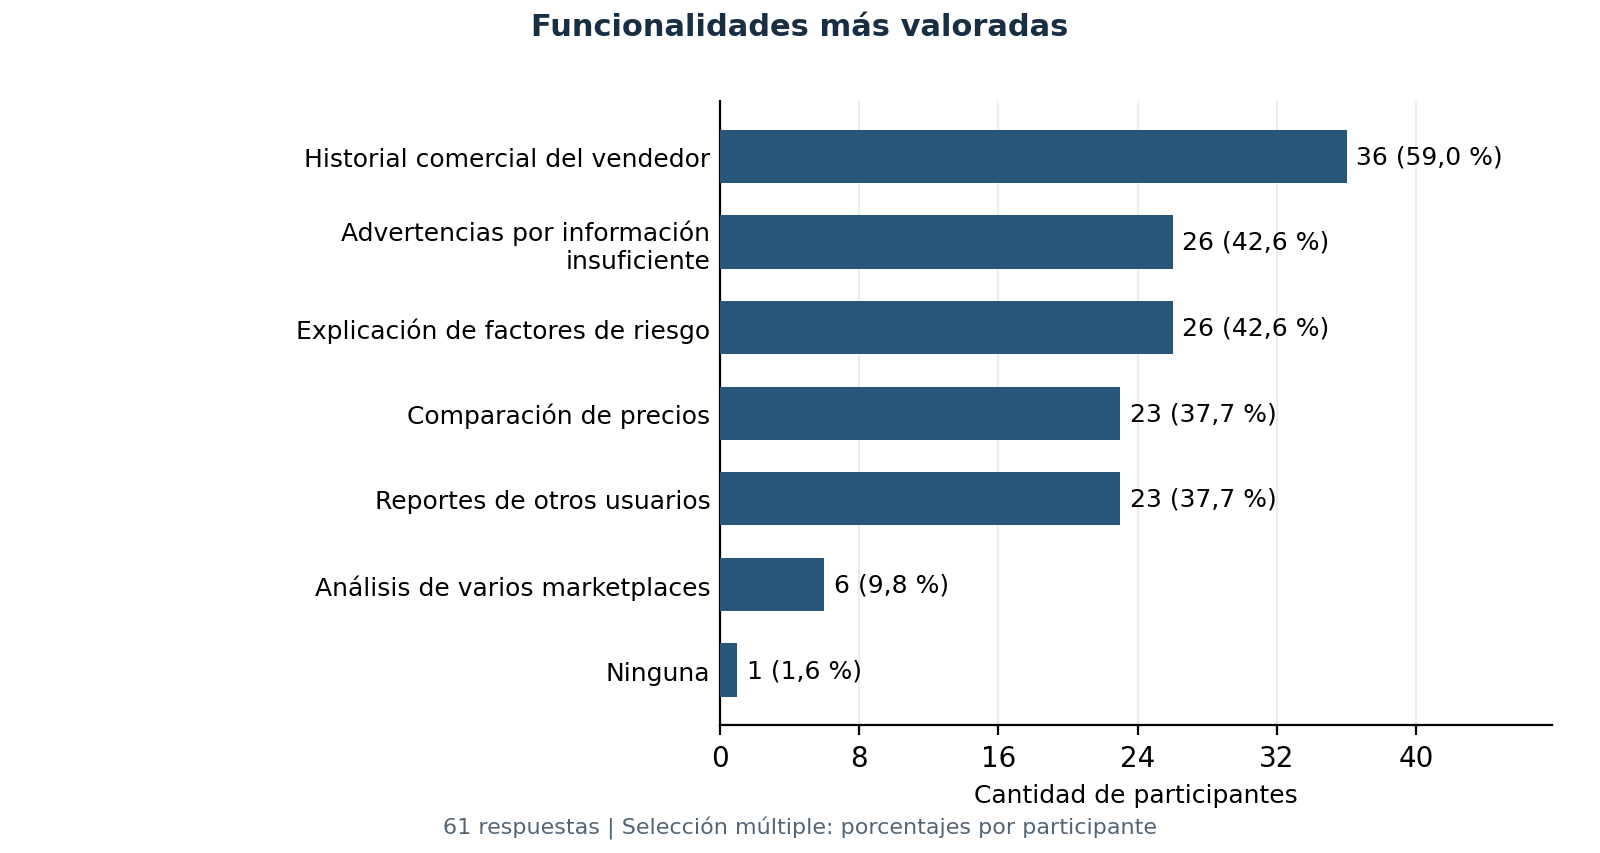
\includegraphics[width=0.94\textwidth,height=0.37\textheight,keepaspectratio]{figuras/marketlens/encuesta/pregunta_10.png}
\caption{Funcionalidades prioritarias para una herramienta de análisis preventivo (n=61).}\label{fig:ml-encuesta-10}
\end{figure}

\begin{figure}[H]
\centering
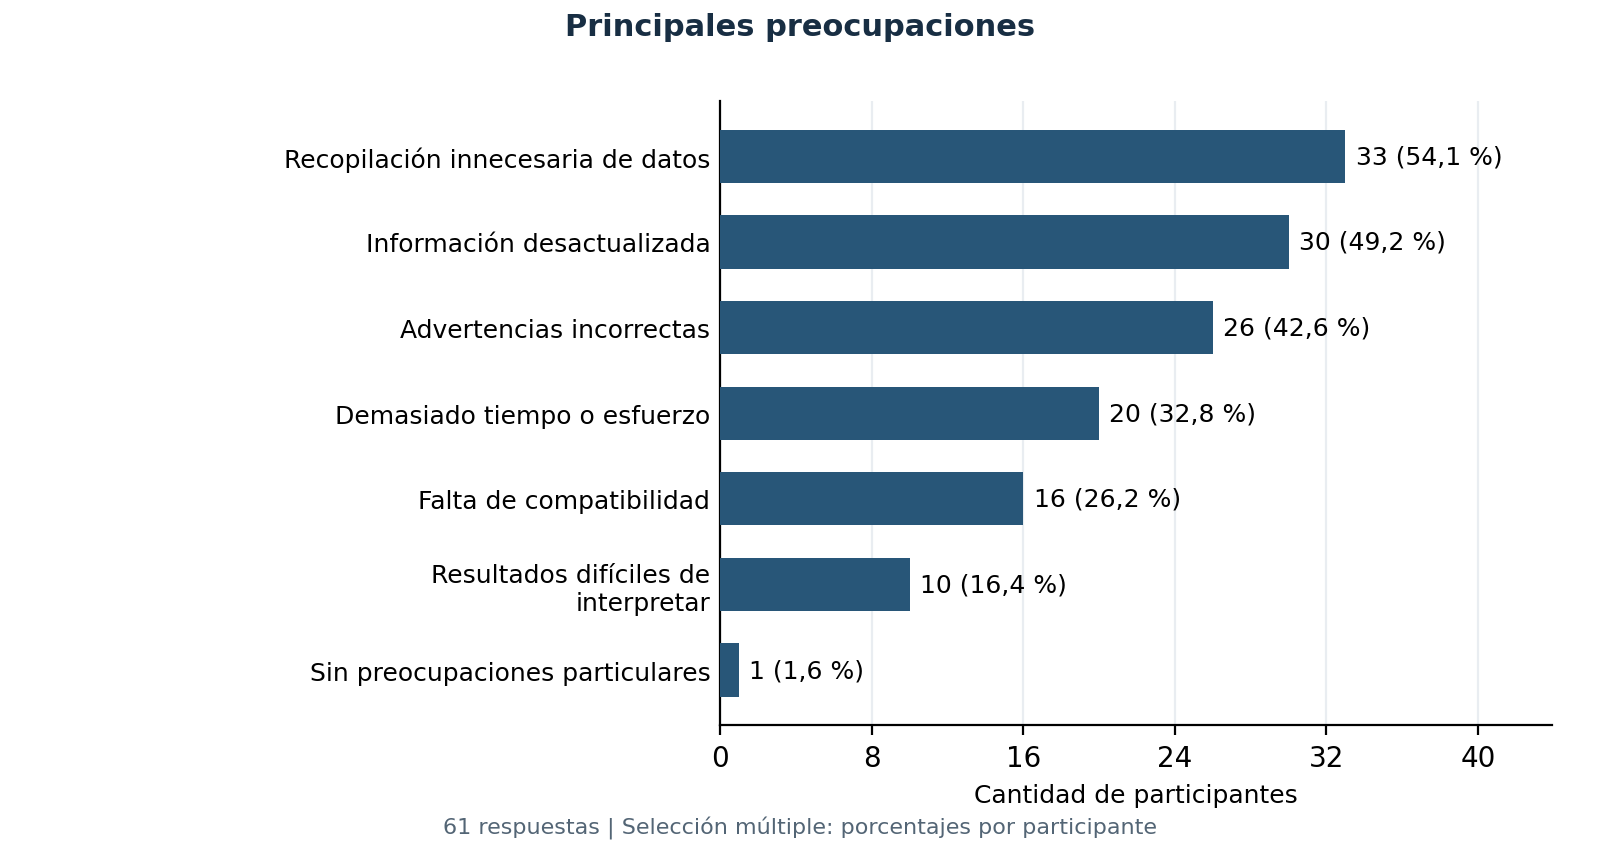
\includegraphics[width=0.94\textwidth,height=0.37\textheight,keepaspectratio]{figuras/marketlens/encuesta/pregunta_11.png}
\caption{Principales preocupaciones respecto del uso de la herramienta (n=61).}\label{fig:ml-encuesta-11}
\end{figure}



\section{Resultados de la encuesta exploratoria}
\label{sec:ml-resultados-encuesta}

Con el propósito de explorar las percepciones de los compradores sobre la seguridad en plataformas digitales y el interés por herramientas preventivas, se aplicó un cuestionario de once preguntas cerradas. El corte de resultados analizado comprende \textbf{61 respuestas} registradas entre el \textbf{10 y el 15 de noviembre de 2026}. El instrumento, sus opciones y las condiciones del relevamiento se incluyen en el apéndice~\ref{apx:encuesta}; el procedimiento se describe en la sección~\ref{subsec:ml-encuesta-metodo}.

La encuesta se difundió mediante contactos del autor y constituye un \textbf{relevamiento exploratorio no probabilístico}. Las cifras expresan percepciones e intenciones declaradas del grupo consultado, sin representatividad estadística de la población general ni evidencia directa de eficacia del motor de detección de fraudes. Las preguntas de selección múltiple admitieron varias alternativas; sus porcentajes se calcularon sobre los 61 participantes y pueden sumar más del 100\,\%.

\begin{table}[H]
\centering
\caption{Síntesis de resultados de la encuesta exploratoria (n=61)}
\label{tab:ml-encuesta-principales}
\small
\begin{tabularx}{\textwidth}{L r r}
\toprule
\tb{Indicador declarado} & \tb{Respuestas} & \tb{Porcentaje} \\
\midrule
Encontró alguna publicación sospechosa & 44/61 & 72,1\,\% \\
Desistió de una compra por desconfianza & 47/61 & 77,0\,\% \\
Calificó la utilidad potencial con 4 o 5 (escala de 1 a 5) & 50/61 & 82,0\,\% \\
Consideraría utilizarla de forma frecuente o ante dudas & 58/61 & 95,1\,\% \\
Asignó 4 o 5 de confianza a los mecanismos actuales & 35/61 & 57,4\,\% \\
\bottomrule
\end{tabularx}
\end{table}

\subsection{Experiencia de compra y criterios de evaluación}

El cuestionario contempló tanto participantes que habían comprado durante los últimos doce meses como otros que no lo habían hecho. El uso de cada plataforma, que podía informarse en conjunto con otras, se presenta en la figura~\ref{fig:ml-encuesta-02}. Mercado Libre fue seleccionado por \textbf{52 personas (85,2\,\%)}. En cuanto a los criterios consultados, los más frecuentes fueron la reputación o calificaciones del vendedor (\textbf{50/61}) y las opiniones de compradores anteriores (\textbf{47/61}), tal como muestra la figura~\ref{fig:ml-encuesta-03}.

\subsection{Percepción de riesgo y confianza}

\textbf{44 participantes (72,1\,\%)} señalaron haber encontrado alguna publicación potencialmente sospechosa (figura~\ref{fig:ml-encuesta-04}), mientras que \textbf{47 (77,0\,\%)} indicaron haber desistido de una compra por desconfianza (figura~\ref{fig:ml-encuesta-05}). Ambas preguntas recogen experiencias autopercibidas: no identifican ni verifican casos reales de fraude.

La confianza en los mecanismos actuales de seguridad y reputación se distribuyó en la escala de 1 a 5, con 35 respuestas en los valores 4 o 5 (\textbf{57,4\,\%}). Entre las características que generaron mayor desconfianza se destacaron el precio considerablemente inferior al de ofertas comparables (\textbf{38 respuestas}), la ausencia de calificaciones u opiniones (\textbf{37}) y la solicitud de pago fuera de la plataforma (\textbf{35}). Se trata de percepciones de los participantes y no de una validación de esos indicadores como predictores de fraude.

\subsection{Utilidad percibida e intención declarada de uso}

Tras presentar una descripción conceptual de una herramienta independiente de análisis preventivo, \textbf{50 participantes (82,0\,\%)} asignaron una utilidad de 4 o 5 en una escala de cinco puntos (figura~\ref{fig:ml-encuesta-08}). Además, \textbf{58 (95,1\,\%)} manifestaron que probablemente utilizarían una herramienta gratuita con frecuencia o ante publicaciones que les generaran dudas (figura~\ref{fig:ml-encuesta-09}). Estas respuestas sugieren \emph{interés declarado} y no constituyen evidencia de adopción efectiva.

En cuanto a funcionalidades, la opción más señalada fue la información sobre el historial comercial del vendedor (\textbf{36 respuestas; 59,0\,\%}). Las advertencias sobre datos insuficientes y la explicación de los factores de riesgo reunieron 26 selecciones cada una. Entre las preocupaciones, destacaron la recopilación innecesaria de datos personales (\textbf{33 respuestas}), la información desactualizada (\textbf{30}) y las advertencias incorrectas (\textbf{26}). Estos resultados sirven para orientar prioridades de transparencia, privacidad y calidad de datos, pero por sí solos no validan decisiones técnicas específicas.

\subsection{Alcance y limitaciones del relevamiento}

La distribución del formulario entre contactos y la participación voluntaria introducen posibles \textbf{sesgos de selección y autoselección}. El instrumento no relevó variables sociodemográficas ni verificó en forma independiente las experiencias declaradas. Por consiguiente, no es posible generalizar los resultados a la totalidad de compradores ni estimar márgenes de error de muestreo probabilístico. Asimismo, la descripción conceptual de MarketLens puede influir en las valoraciones de utilidad e intención de uso.

Estas evidencias complementan la justificación del problema abordado y permiten identificar prioridades expresadas por las personas encuestadas. No deben confundirse con pruebas de usabilidad del prototipo, validaciones de precisión del índice de riesgo o una medición de su impacto real en la prevención de estafas. El presente corte corresponde a 61 respuestas; de incorporarse nuevas respuestas, deben recalcularse todos los porcentajes y sustituirse los gráficos correspondientes.

\subsection{Distribución completa de respuestas}

Las figuras siguientes presentan las frecuencias absolutas y los porcentajes observados para las once preguntas, incluida la opción de valoración no seleccionada en las escalas. En preguntas de selección múltiple, el denominador continúa siendo el número total de participantes (61).
\begin{figure}[H]
\centering
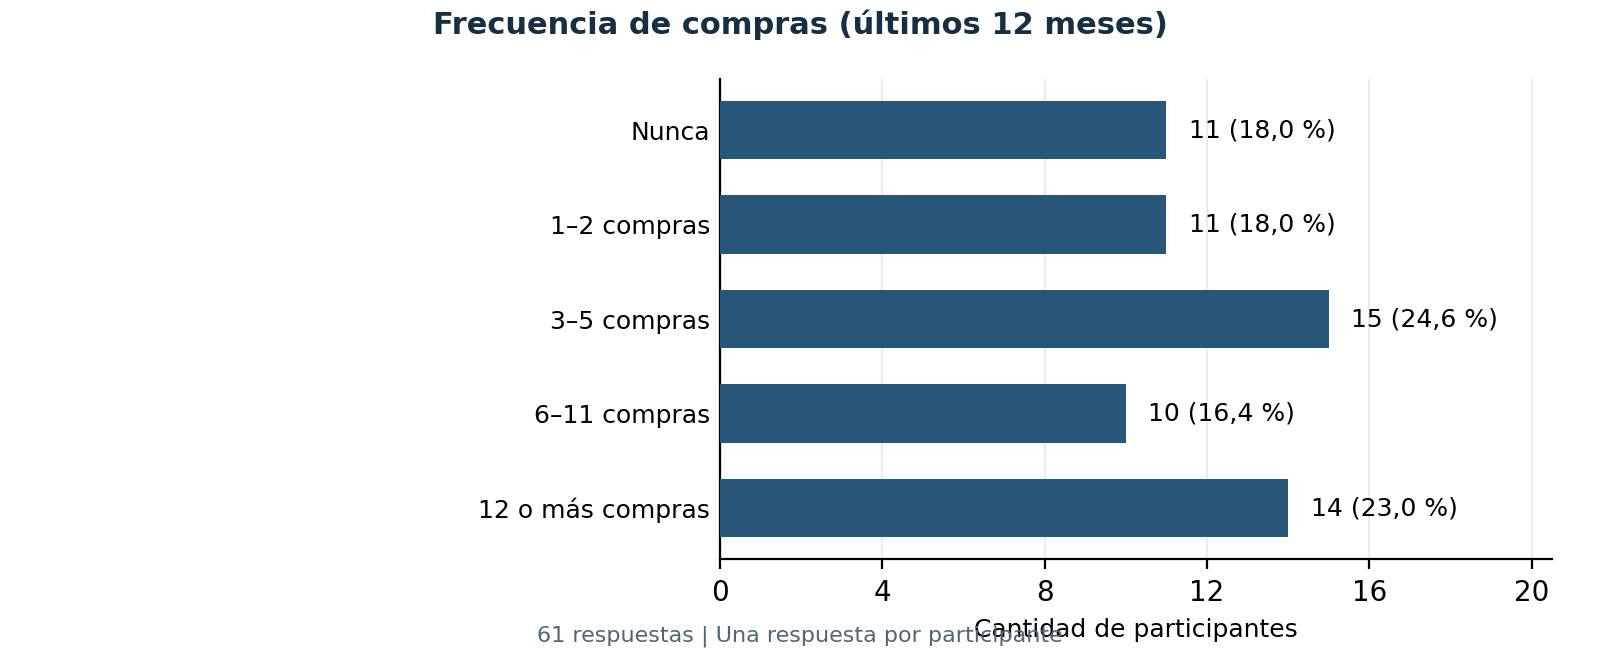
\includegraphics[width=0.94\textwidth,height=0.37\textheight,keepaspectratio]{figuras/marketlens/encuesta/pregunta_01.png}
\caption{Frecuencia de compra declarada en marketplaces durante los últimos doce meses (n=61).}\label{fig:ml-encuesta-01}
\end{figure}

\begin{figure}[H]
\centering
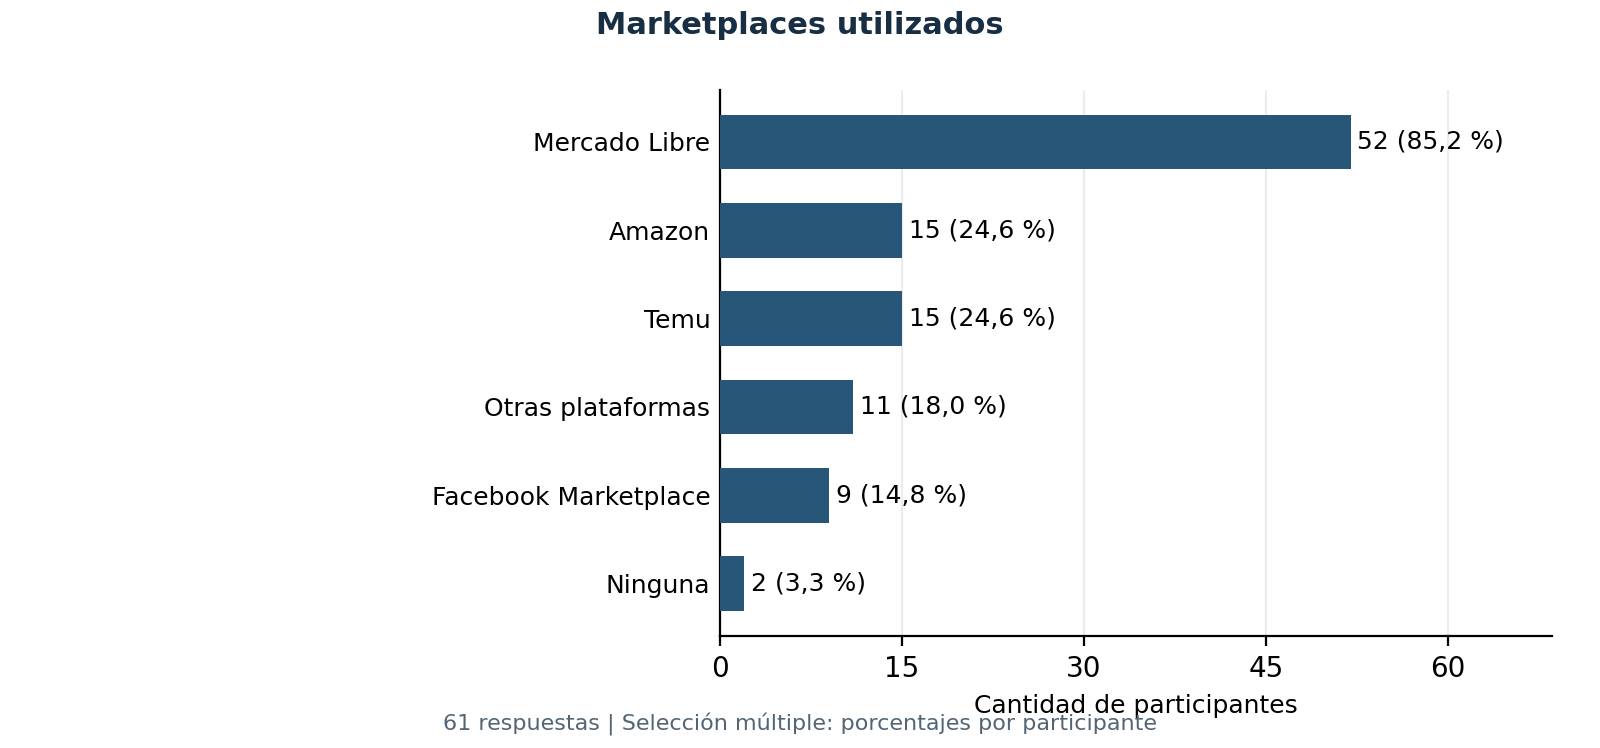
\includegraphics[width=0.94\textwidth,height=0.37\textheight,keepaspectratio]{figuras/marketlens/encuesta/pregunta_02.png}
\caption{Plataformas utilizadas por los encuestados durante los últimos doce meses (n=61).}\label{fig:ml-encuesta-02}
\end{figure}

\begin{figure}[H]
\centering
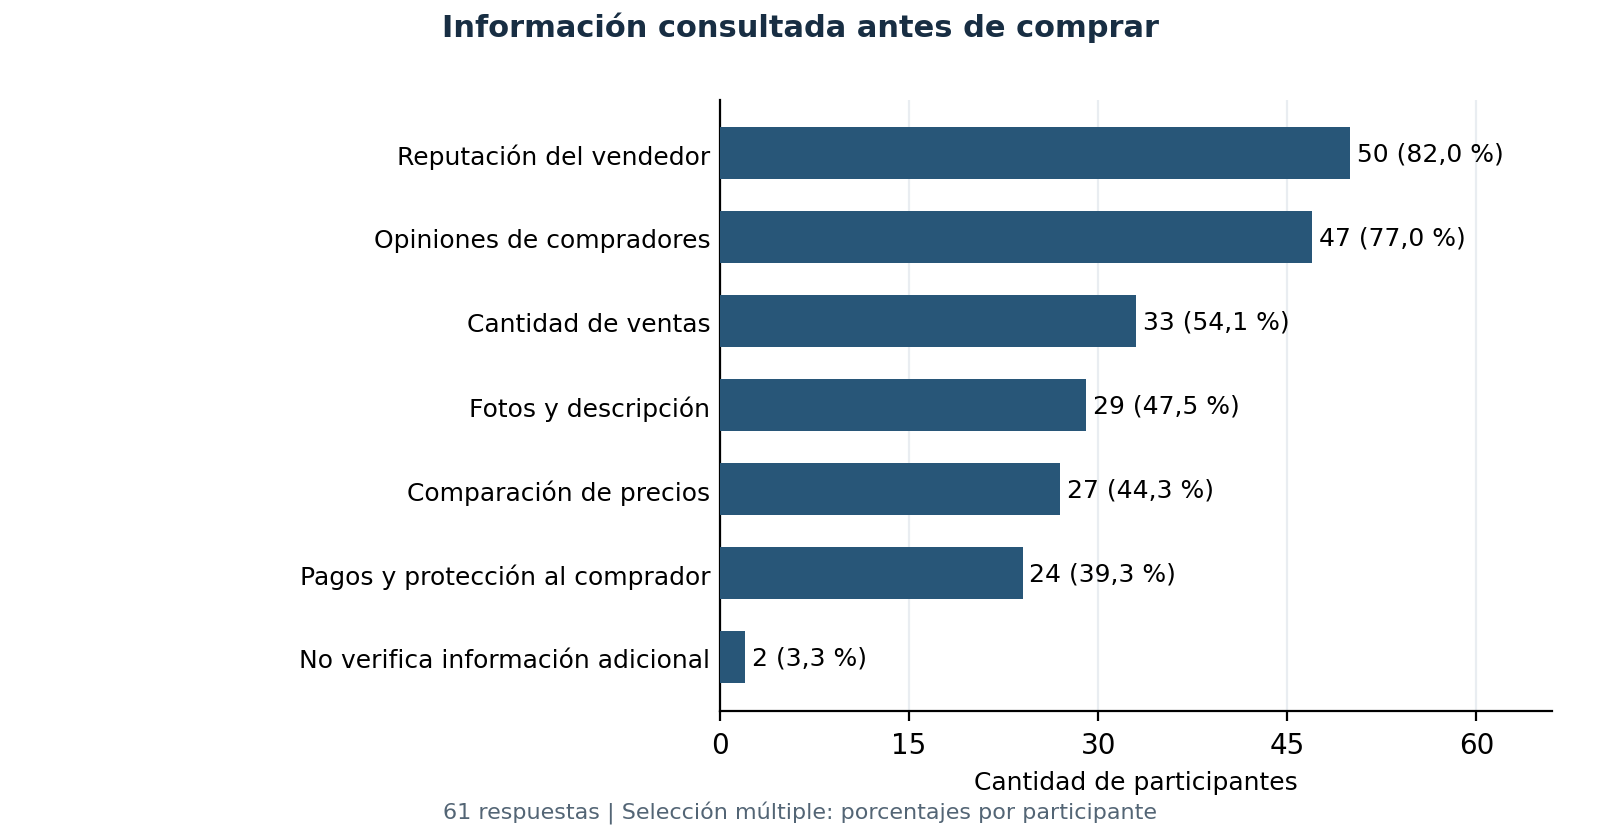
\includegraphics[width=0.94\textwidth,height=0.37\textheight,keepaspectratio]{figuras/marketlens/encuesta/pregunta_03.png}
\caption{Información habitualmente consultada para evaluar publicaciones o vendedores (n=61).}\label{fig:ml-encuesta-03}
\end{figure}

\begin{figure}[H]
\centering
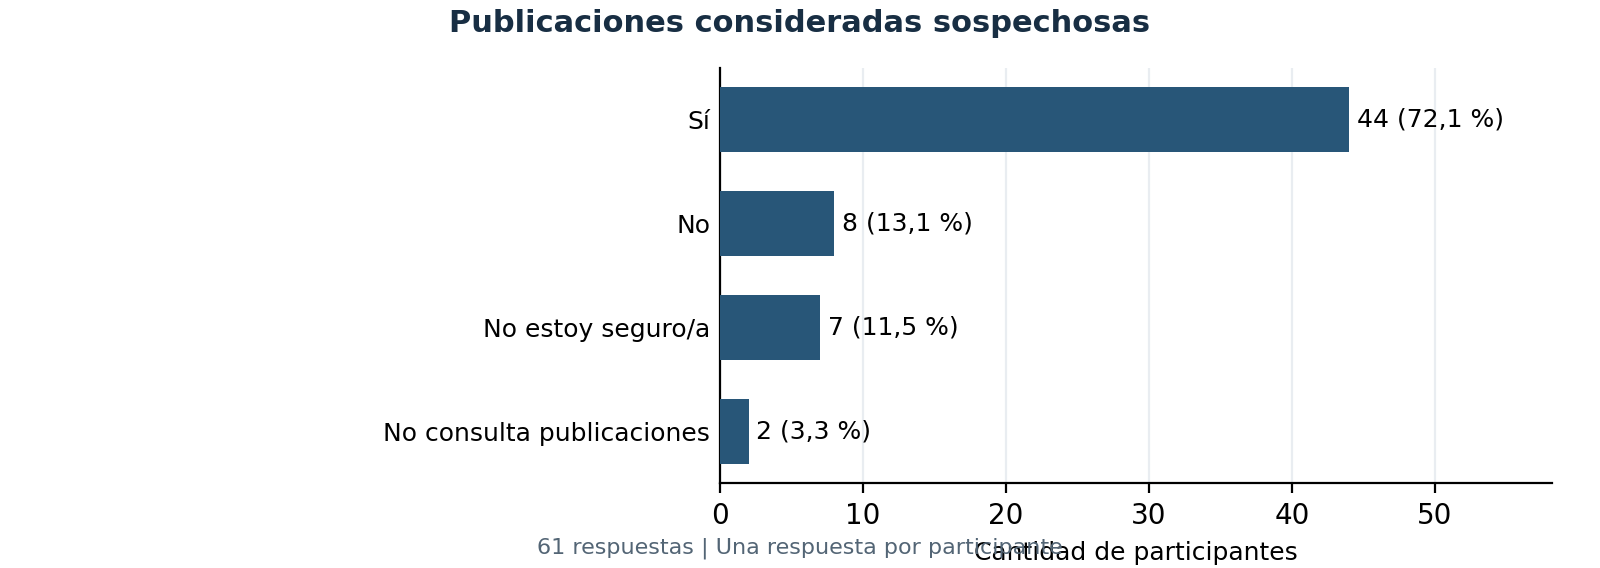
\includegraphics[width=0.94\textwidth,height=0.37\textheight,keepaspectratio]{figuras/marketlens/encuesta/pregunta_04.png}
\caption{Encuestados que identificaron publicaciones potencialmente sospechosas (n=61).}\label{fig:ml-encuesta-04}
\end{figure}

\begin{figure}[H]
\centering
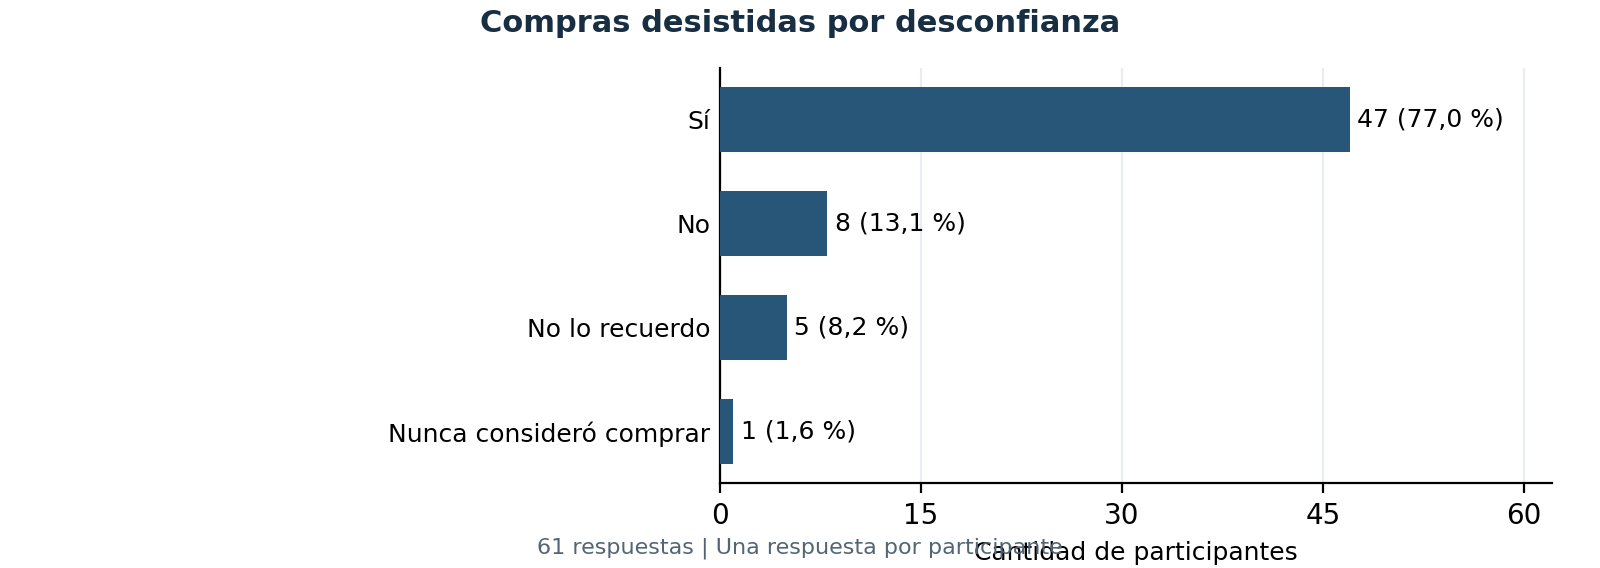
\includegraphics[width=0.94\textwidth,height=0.37\textheight,keepaspectratio]{figuras/marketlens/encuesta/pregunta_05.png}
\caption{Encuestados que desistieron de una compra por desconfianza (n=61).}\label{fig:ml-encuesta-05}
\end{figure}

\begin{figure}[H]
\centering
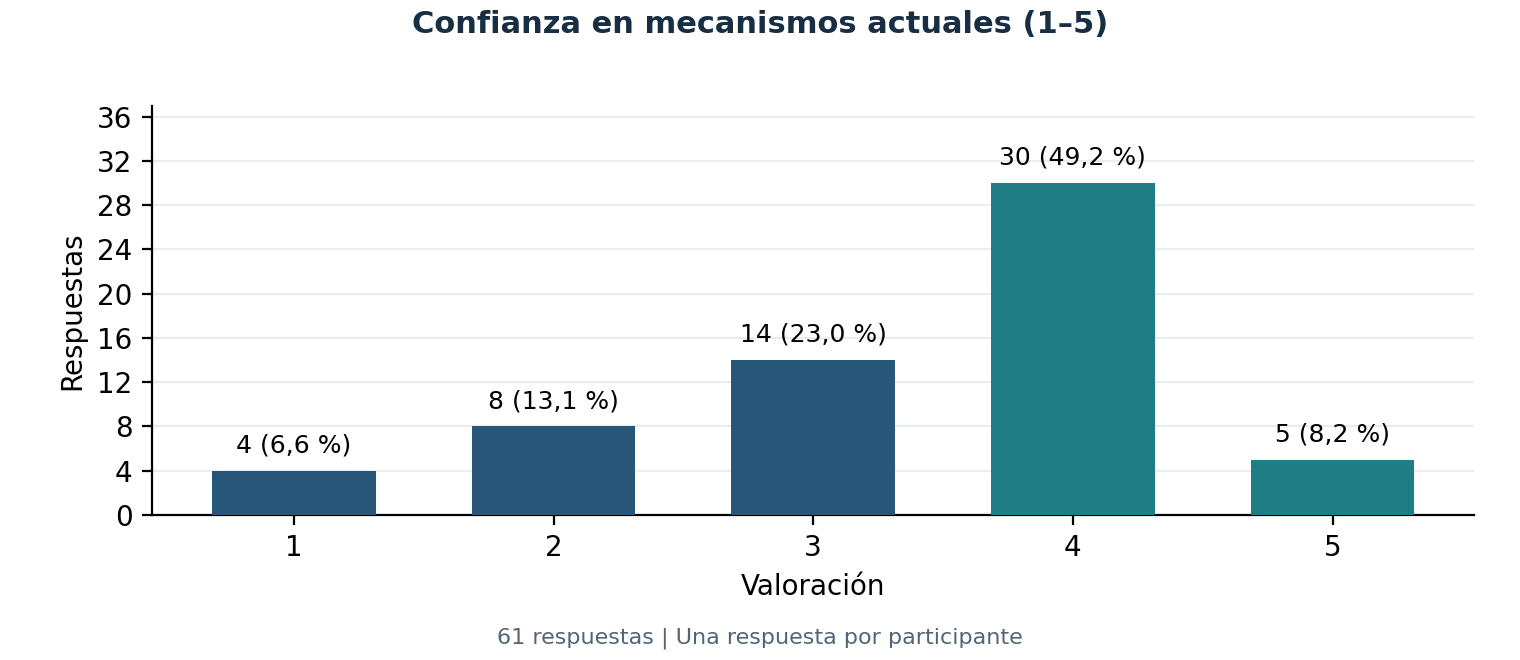
\includegraphics[width=0.94\textwidth,height=0.37\textheight,keepaspectratio]{figuras/marketlens/encuesta/pregunta_06.png}
\caption{Confianza declarada en los mecanismos actuales de seguridad y reputación (n=61).}\label{fig:ml-encuesta-06}
\end{figure}

\begin{figure}[H]
\centering
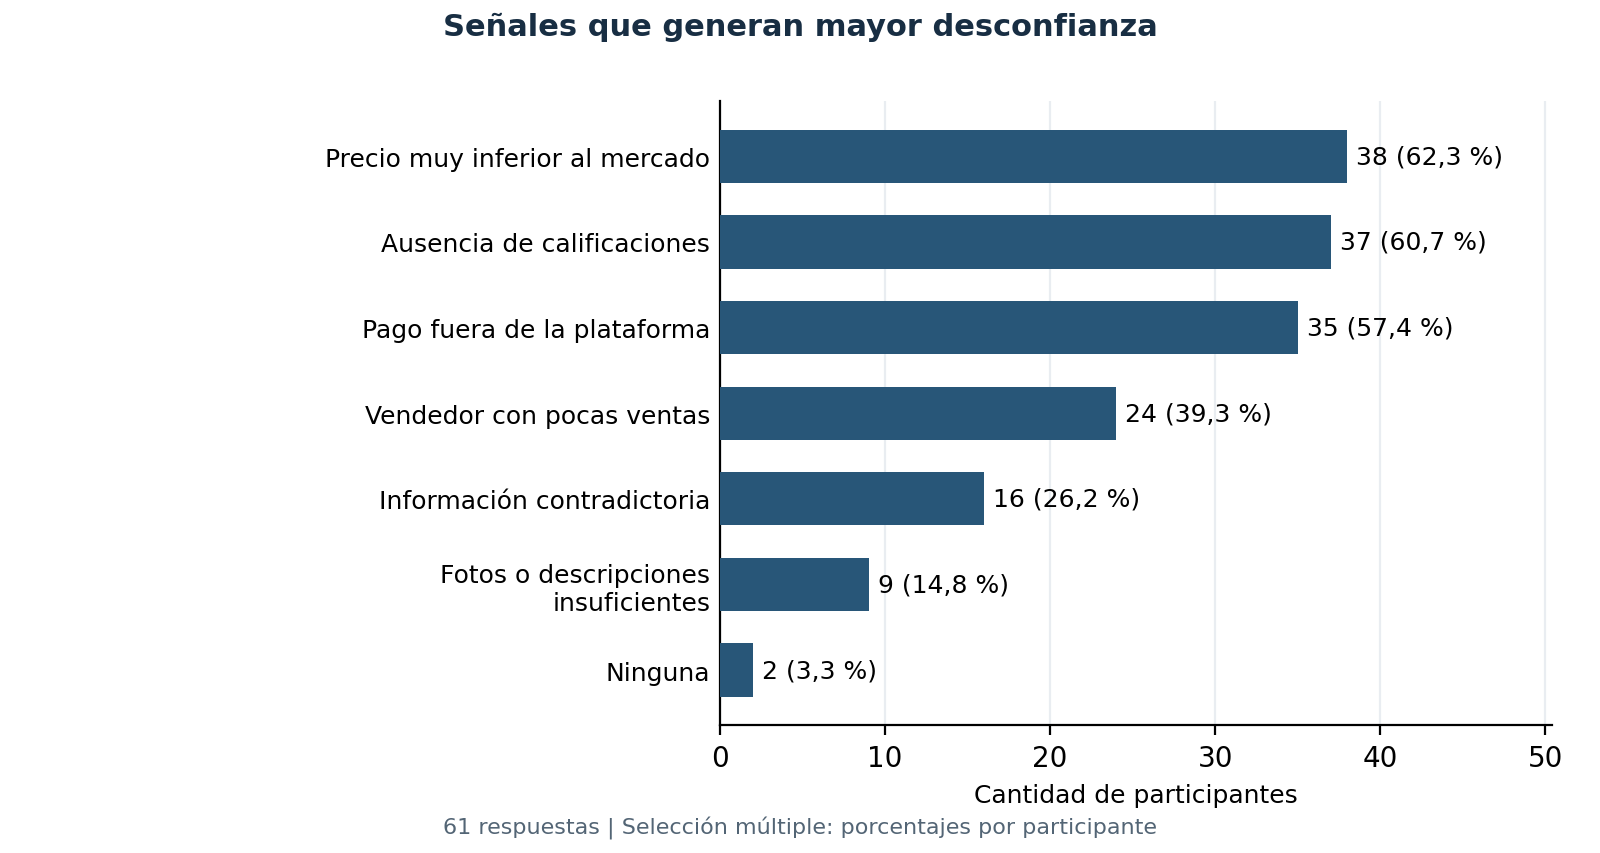
\includegraphics[width=0.94\textwidth,height=0.37\textheight,keepaspectratio]{figuras/marketlens/encuesta/pregunta_07.png}
\caption{Características de publicaciones que generan mayor desconfianza (n=61).}\label{fig:ml-encuesta-07}
\end{figure}

\begin{figure}[H]
\centering
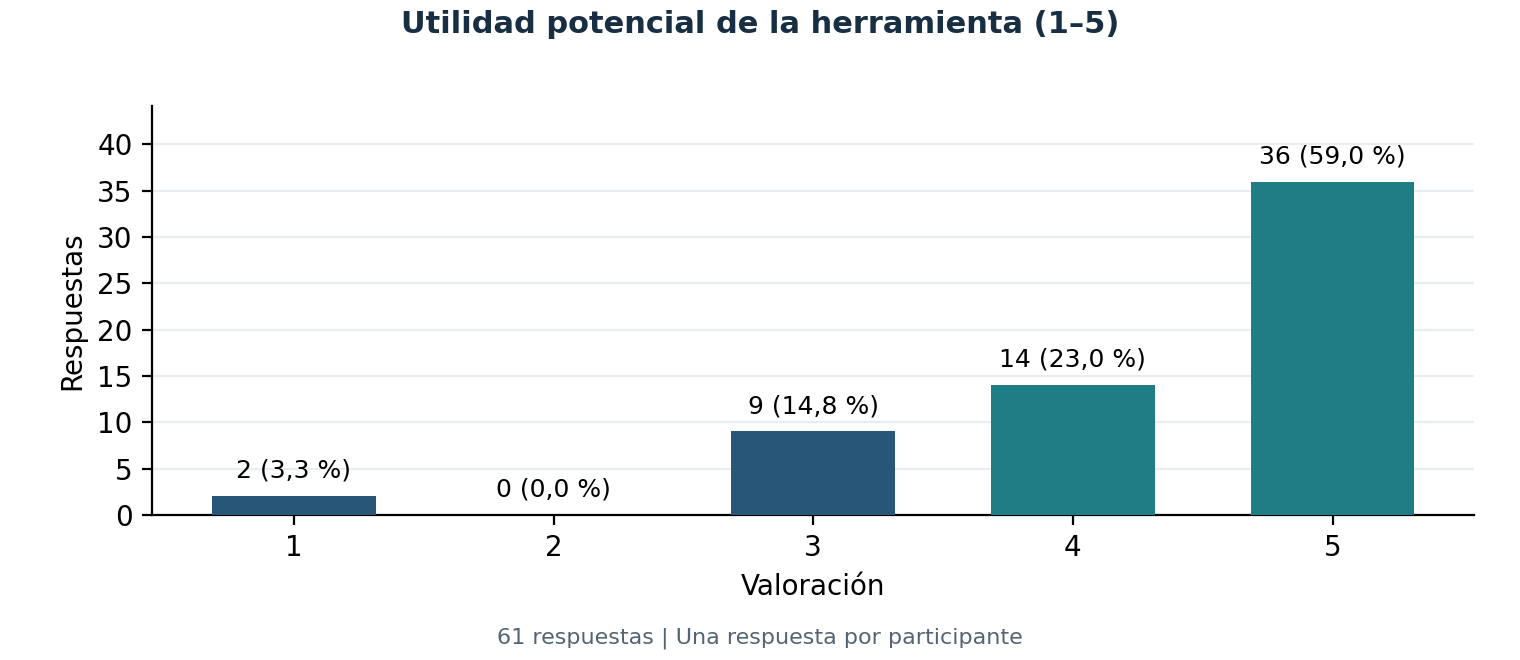
\includegraphics[width=0.94\textwidth,height=0.37\textheight,keepaspectratio]{figuras/marketlens/encuesta/pregunta_08.png}
\caption{Utilidad potencial atribuida a una herramienta de análisis preventivo (n=61).}\label{fig:ml-encuesta-08}
\end{figure}

\begin{figure}[H]
\centering
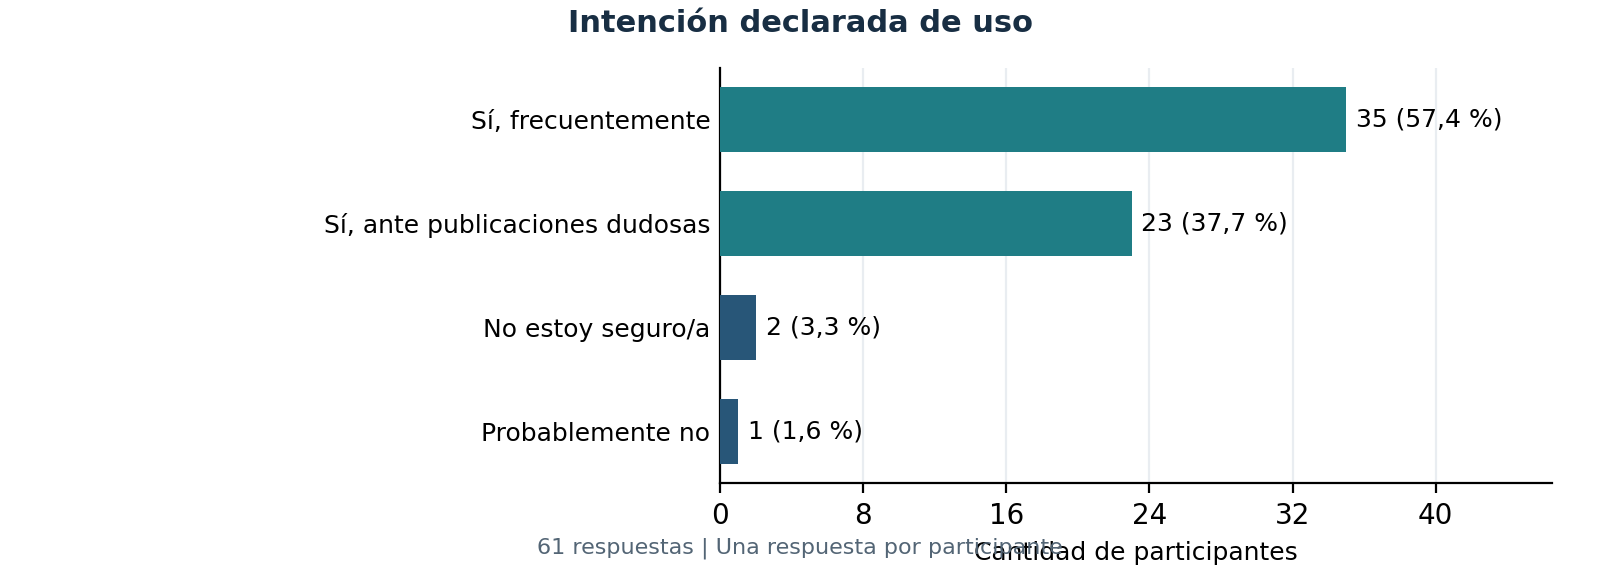
\includegraphics[width=0.94\textwidth,height=0.37\textheight,keepaspectratio]{figuras/marketlens/encuesta/pregunta_09.png}
\caption{Intención declarada de utilización de una herramienta gratuita como la propuesta (n=61).}\label{fig:ml-encuesta-09}
\end{figure}

\begin{figure}[H]
\centering
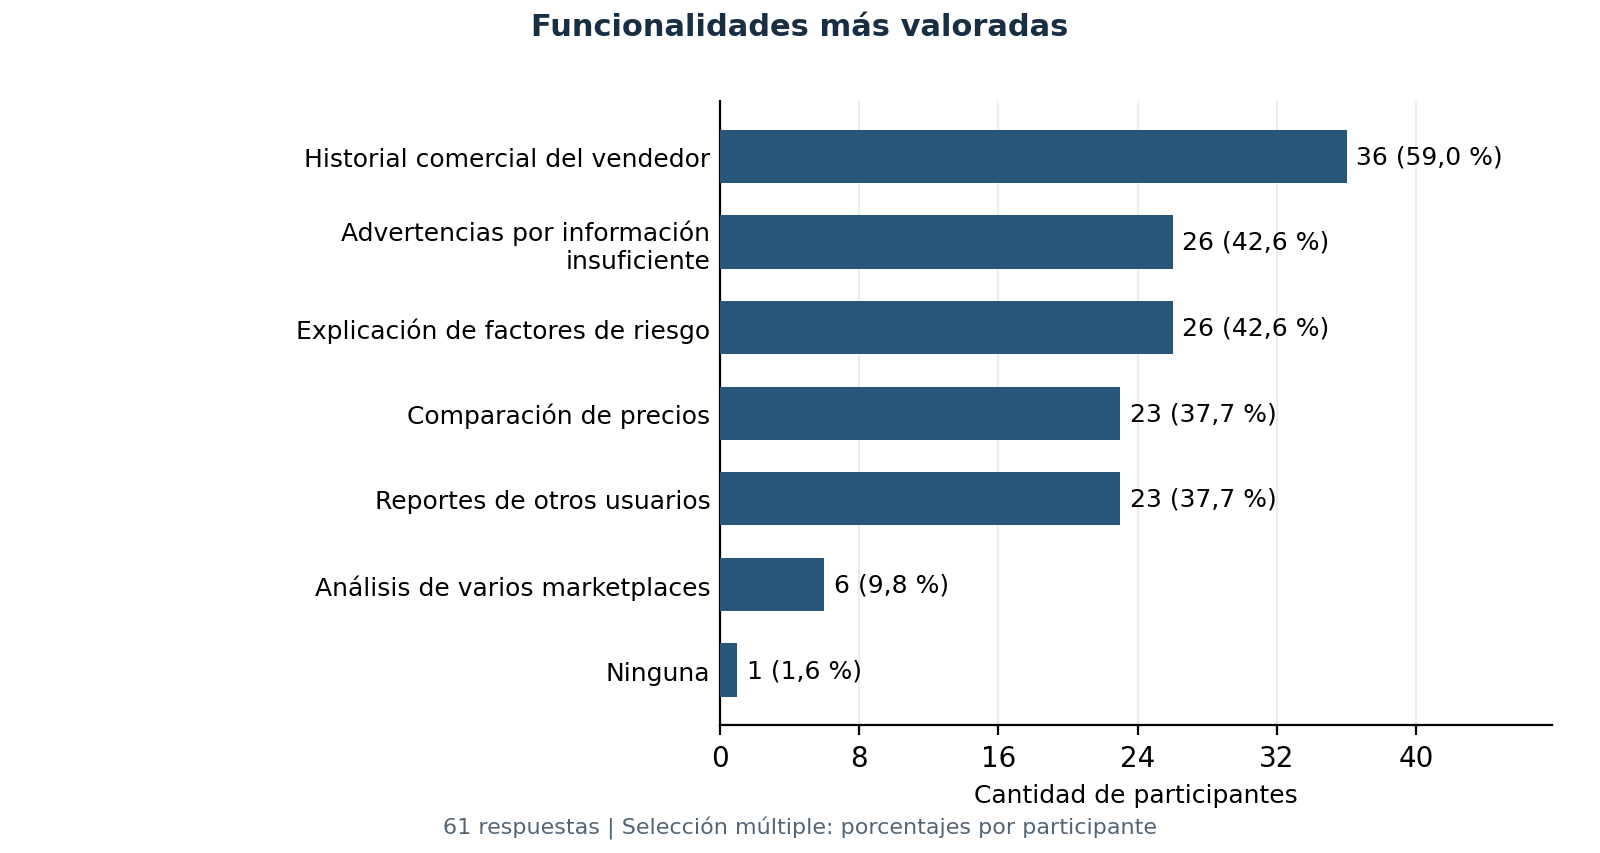
\includegraphics[width=0.94\textwidth,height=0.37\textheight,keepaspectratio]{figuras/marketlens/encuesta/pregunta_10.png}
\caption{Funcionalidades prioritarias para una herramienta de análisis preventivo (n=61).}\label{fig:ml-encuesta-10}
\end{figure}

\begin{figure}[H]
\centering
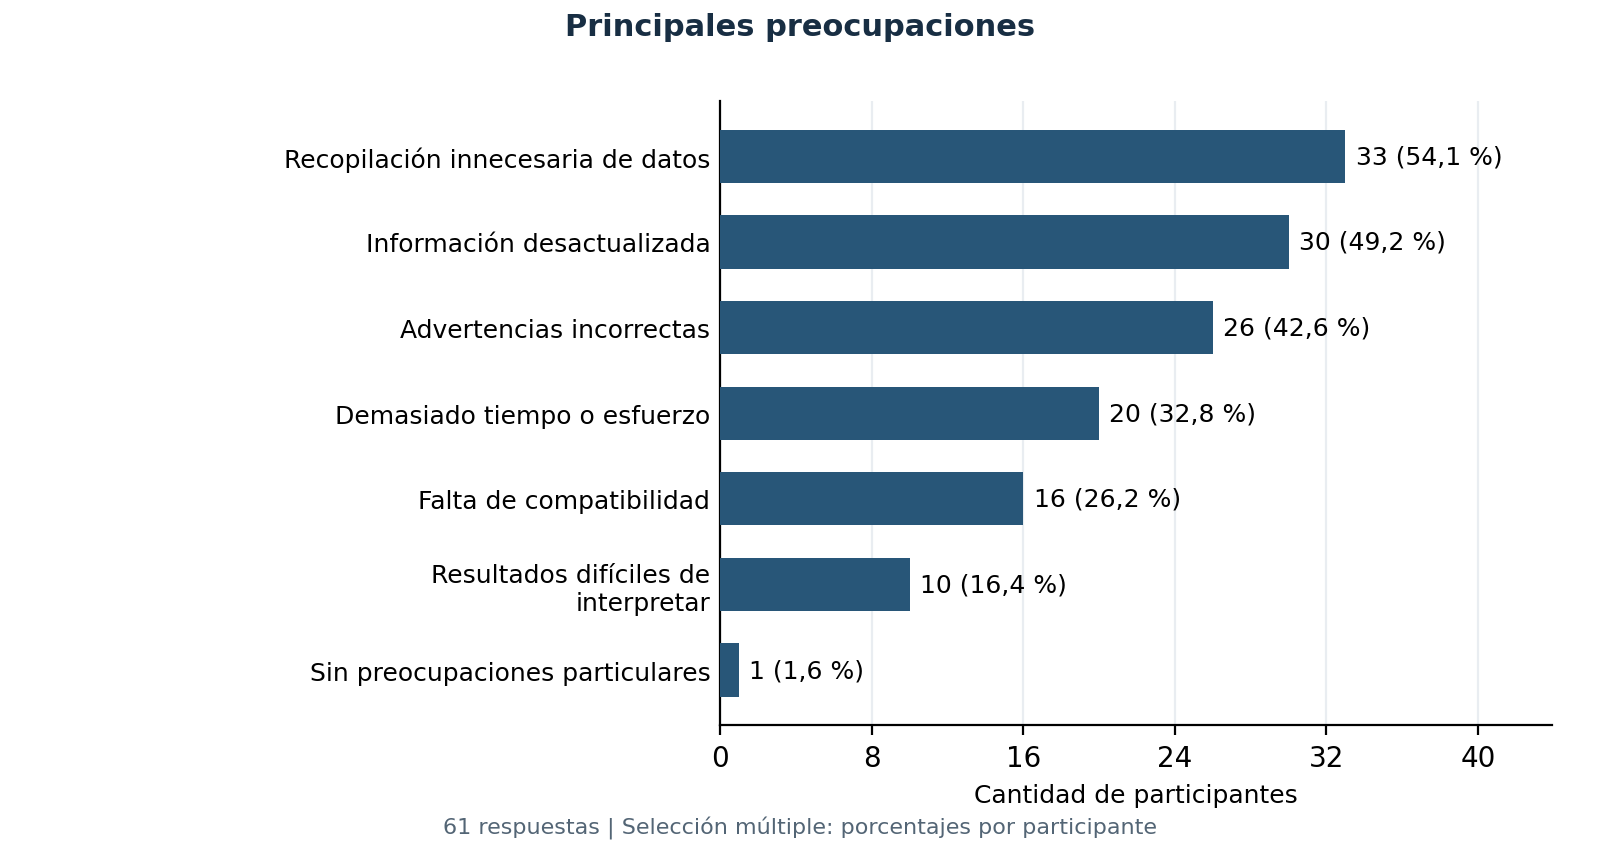
\includegraphics[width=0.94\textwidth,height=0.37\textheight,keepaspectratio]{figuras/marketlens/encuesta/pregunta_11.png}
\caption{Principales preocupaciones respecto del uso de la herramienta (n=61).}\label{fig:ml-encuesta-11}
\end{figure}



\section{Resultados de la encuesta exploratoria}
\label{sec:ml-resultados-encuesta}

Con el propósito de explorar las percepciones de los compradores sobre la seguridad en plataformas digitales y el interés por herramientas preventivas, se aplicó un cuestionario de once preguntas cerradas. El corte de resultados analizado comprende \textbf{61 respuestas} registradas entre el \textbf{10 y el 15 de noviembre de 2026}. El instrumento, sus opciones y las condiciones del relevamiento se incluyen en el apéndice~\ref{apx:encuesta}; el procedimiento se describe en la sección~\ref{subsec:ml-encuesta-metodo}.

La encuesta se difundió mediante contactos del autor y constituye un \textbf{relevamiento exploratorio no probabilístico}. Las cifras expresan percepciones e intenciones declaradas del grupo consultado, sin representatividad estadística de la población general ni evidencia directa de eficacia del motor de detección de fraudes. Las preguntas de selección múltiple admitieron varias alternativas; sus porcentajes se calcularon sobre los 61 participantes y pueden sumar más del 100\,\%.

\begin{table}[H]
\centering
\caption{Síntesis de resultados de la encuesta exploratoria (n=61)}
\label{tab:ml-encuesta-principales}
\small
\begin{tabularx}{\textwidth}{L r r}
\toprule
\tb{Indicador declarado} & \tb{Respuestas} & \tb{Porcentaje} \\
\midrule
Encontró alguna publicación sospechosa & 44/61 & 72,1\,\% \\
Desistió de una compra por desconfianza & 47/61 & 77,0\,\% \\
Calificó la utilidad potencial con 4 o 5 (escala de 1 a 5) & 50/61 & 82,0\,\% \\
Consideraría utilizarla de forma frecuente o ante dudas & 58/61 & 95,1\,\% \\
Asignó 4 o 5 de confianza a los mecanismos actuales & 35/61 & 57,4\,\% \\
\bottomrule
\end{tabularx}
\end{table}

\subsection{Experiencia de compra y criterios de evaluación}

El cuestionario contempló tanto participantes que habían comprado durante los últimos doce meses como otros que no lo habían hecho. El uso de cada plataforma, que podía informarse en conjunto con otras, se presenta en la figura~\ref{fig:ml-encuesta-02}. Mercado Libre fue seleccionado por \textbf{52 personas (85,2\,\%)}. En cuanto a los criterios consultados, los más frecuentes fueron la reputación o calificaciones del vendedor (\textbf{50/61}) y las opiniones de compradores anteriores (\textbf{47/61}), tal como muestra la figura~\ref{fig:ml-encuesta-03}.

\subsection{Percepción de riesgo y confianza}

\textbf{44 participantes (72,1\,\%)} señalaron haber encontrado alguna publicación potencialmente sospechosa (figura~\ref{fig:ml-encuesta-04}), mientras que \textbf{47 (77,0\,\%)} indicaron haber desistido de una compra por desconfianza (figura~\ref{fig:ml-encuesta-05}). Ambas preguntas recogen experiencias autopercibidas: no identifican ni verifican casos reales de fraude.

La confianza en los mecanismos actuales de seguridad y reputación se distribuyó en la escala de 1 a 5, con 35 respuestas en los valores 4 o 5 (\textbf{57,4\,\%}). Entre las características que generaron mayor desconfianza se destacaron el precio considerablemente inferior al de ofertas comparables (\textbf{38 respuestas}), la ausencia de calificaciones u opiniones (\textbf{37}) y la solicitud de pago fuera de la plataforma (\textbf{35}). Se trata de percepciones de los participantes y no de una validación de esos indicadores como predictores de fraude.

\subsection{Utilidad percibida e intención declarada de uso}

Tras presentar una descripción conceptual de una herramienta independiente de análisis preventivo, \textbf{50 participantes (82,0\,\%)} asignaron una utilidad de 4 o 5 en una escala de cinco puntos (figura~\ref{fig:ml-encuesta-08}). Además, \textbf{58 (95,1\,\%)} manifestaron que probablemente utilizarían una herramienta gratuita con frecuencia o ante publicaciones que les generaran dudas (figura~\ref{fig:ml-encuesta-09}). Estas respuestas sugieren \emph{interés declarado} y no constituyen evidencia de adopción efectiva.

En cuanto a funcionalidades, la opción más señalada fue la información sobre el historial comercial del vendedor (\textbf{36 respuestas; 59,0\,\%}). Las advertencias sobre datos insuficientes y la explicación de los factores de riesgo reunieron 26 selecciones cada una. Entre las preocupaciones, destacaron la recopilación innecesaria de datos personales (\textbf{33 respuestas}), la información desactualizada (\textbf{30}) y las advertencias incorrectas (\textbf{26}). Estos resultados sirven para orientar prioridades de transparencia, privacidad y calidad de datos, pero por sí solos no validan decisiones técnicas específicas.

\subsection{Alcance y limitaciones del relevamiento}

La distribución del formulario entre contactos y la participación voluntaria introducen posibles \textbf{sesgos de selección y autoselección}. El instrumento no relevó variables sociodemográficas ni verificó en forma independiente las experiencias declaradas. Por consiguiente, no es posible generalizar los resultados a la totalidad de compradores ni estimar márgenes de error de muestreo probabilístico. Asimismo, la descripción conceptual de MarketLens puede influir en las valoraciones de utilidad e intención de uso.

Estas evidencias complementan la justificación del problema abordado y permiten identificar prioridades expresadas por las personas encuestadas. No deben confundirse con pruebas de usabilidad del prototipo, validaciones de precisión del índice de riesgo o una medición de su impacto real en la prevención de estafas. El presente corte corresponde a 61 respuestas; de incorporarse nuevas respuestas, deben recalcularse todos los porcentajes y sustituirse los gráficos correspondientes.

\subsection{Distribución completa de respuestas}

Las figuras siguientes presentan las frecuencias absolutas y los porcentajes observados para las once preguntas, incluida la opción de valoración no seleccionada en las escalas. En preguntas de selección múltiple, el denominador continúa siendo el número total de participantes (61).
\begin{figure}[H]
\centering
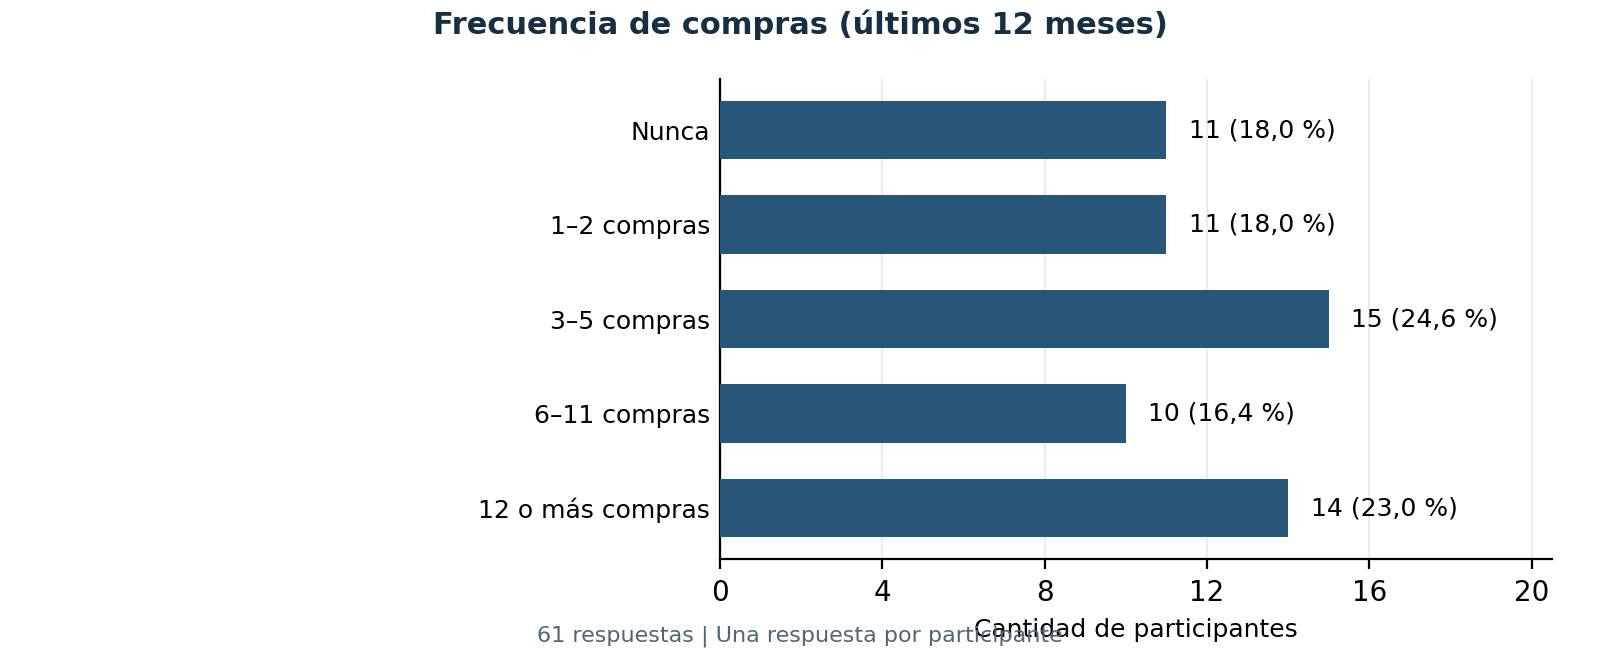
\includegraphics[width=0.94\textwidth,height=0.37\textheight,keepaspectratio]{figuras/marketlens/encuesta/pregunta_01.png}
\caption{Frecuencia de compra declarada en marketplaces durante los últimos doce meses (n=61).}\label{fig:ml-encuesta-01}
\end{figure}

\begin{figure}[H]
\centering
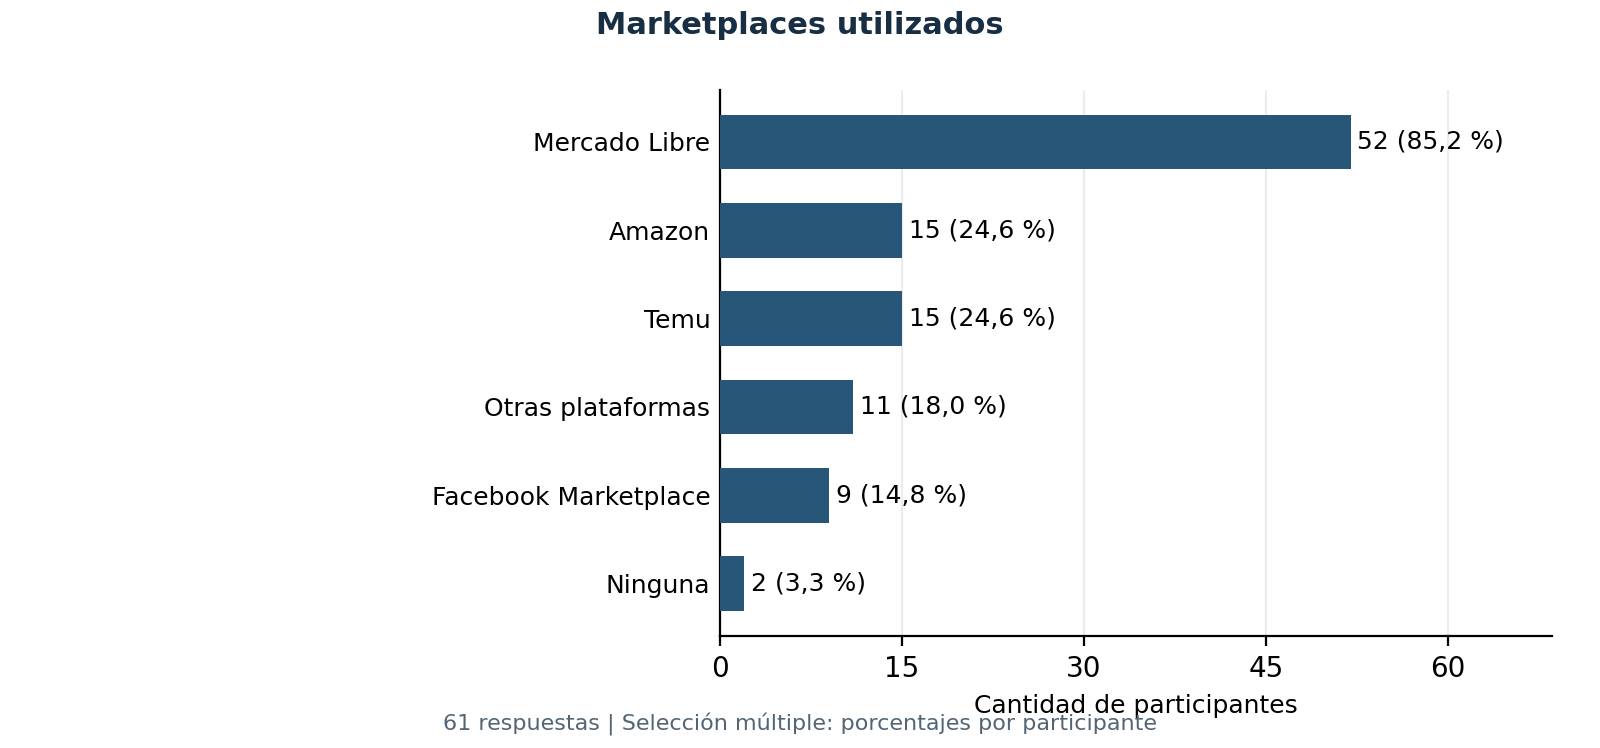
\includegraphics[width=0.94\textwidth,height=0.37\textheight,keepaspectratio]{figuras/marketlens/encuesta/pregunta_02.png}
\caption{Plataformas utilizadas por los encuestados durante los últimos doce meses (n=61).}\label{fig:ml-encuesta-02}
\end{figure}

\begin{figure}[H]
\centering
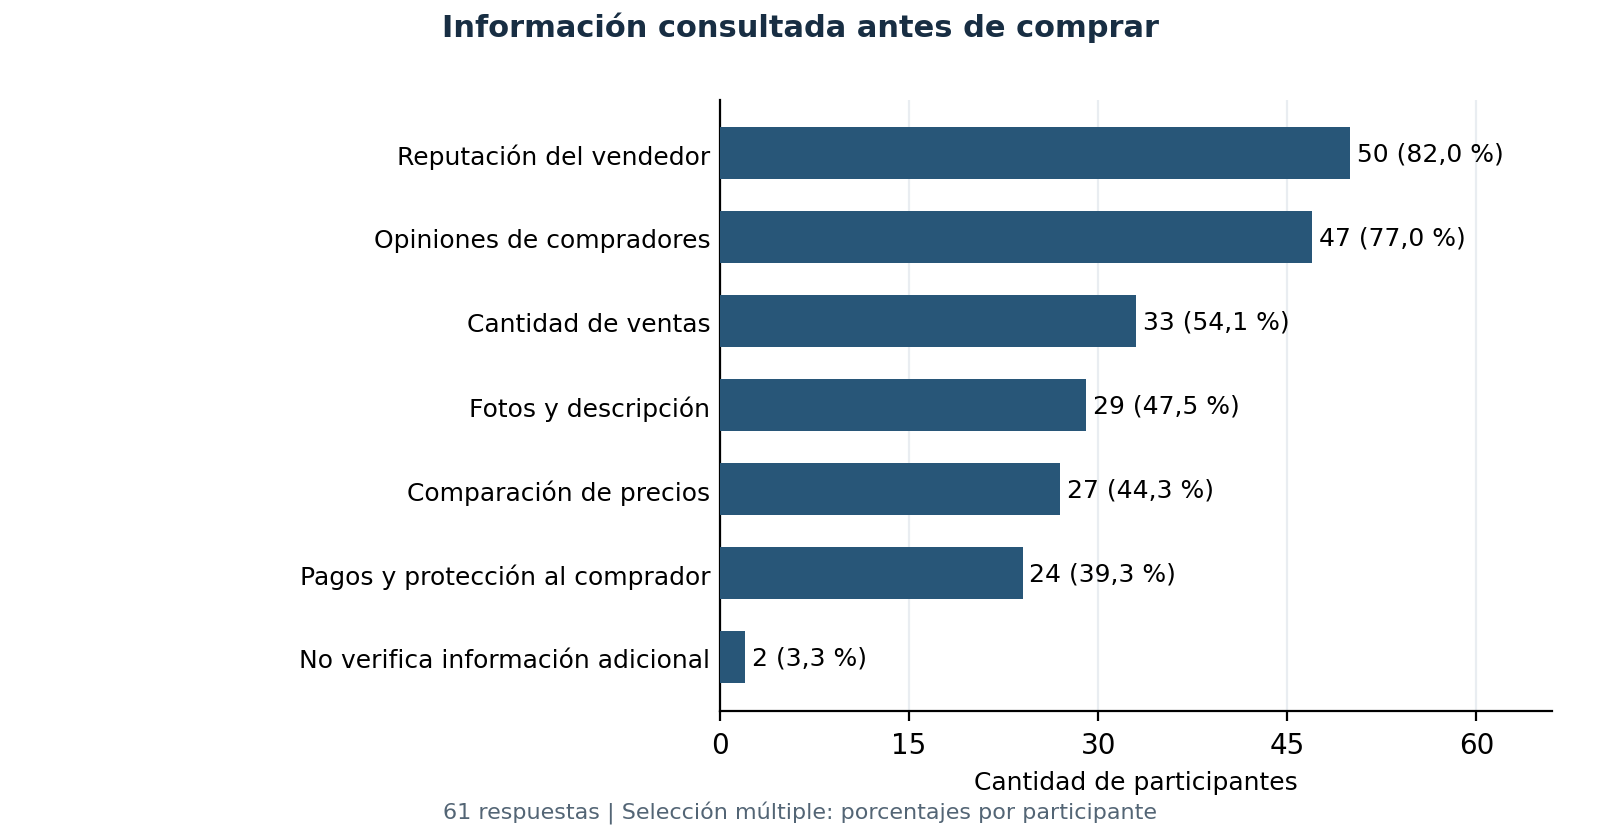
\includegraphics[width=0.94\textwidth,height=0.37\textheight,keepaspectratio]{figuras/marketlens/encuesta/pregunta_03.png}
\caption{Información habitualmente consultada para evaluar publicaciones o vendedores (n=61).}\label{fig:ml-encuesta-03}
\end{figure}

\begin{figure}[H]
\centering
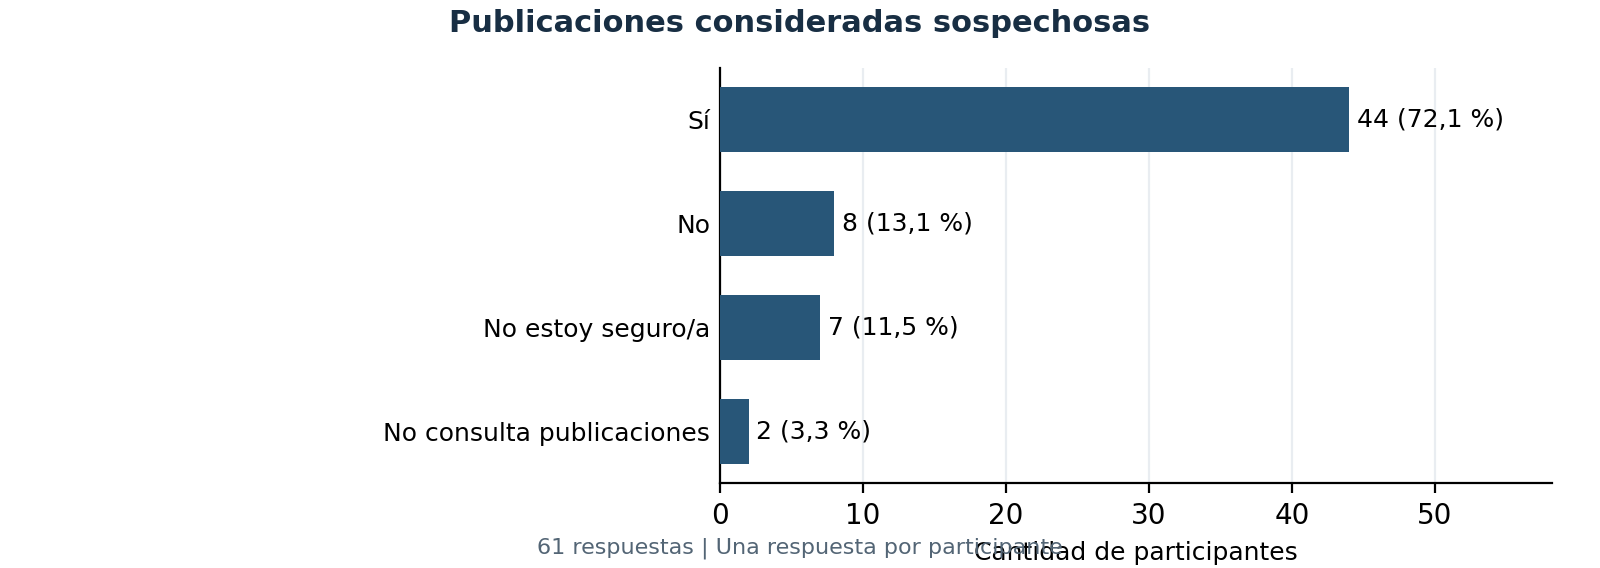
\includegraphics[width=0.94\textwidth,height=0.37\textheight,keepaspectratio]{figuras/marketlens/encuesta/pregunta_04.png}
\caption{Encuestados que identificaron publicaciones potencialmente sospechosas (n=61).}\label{fig:ml-encuesta-04}
\end{figure}

\begin{figure}[H]
\centering
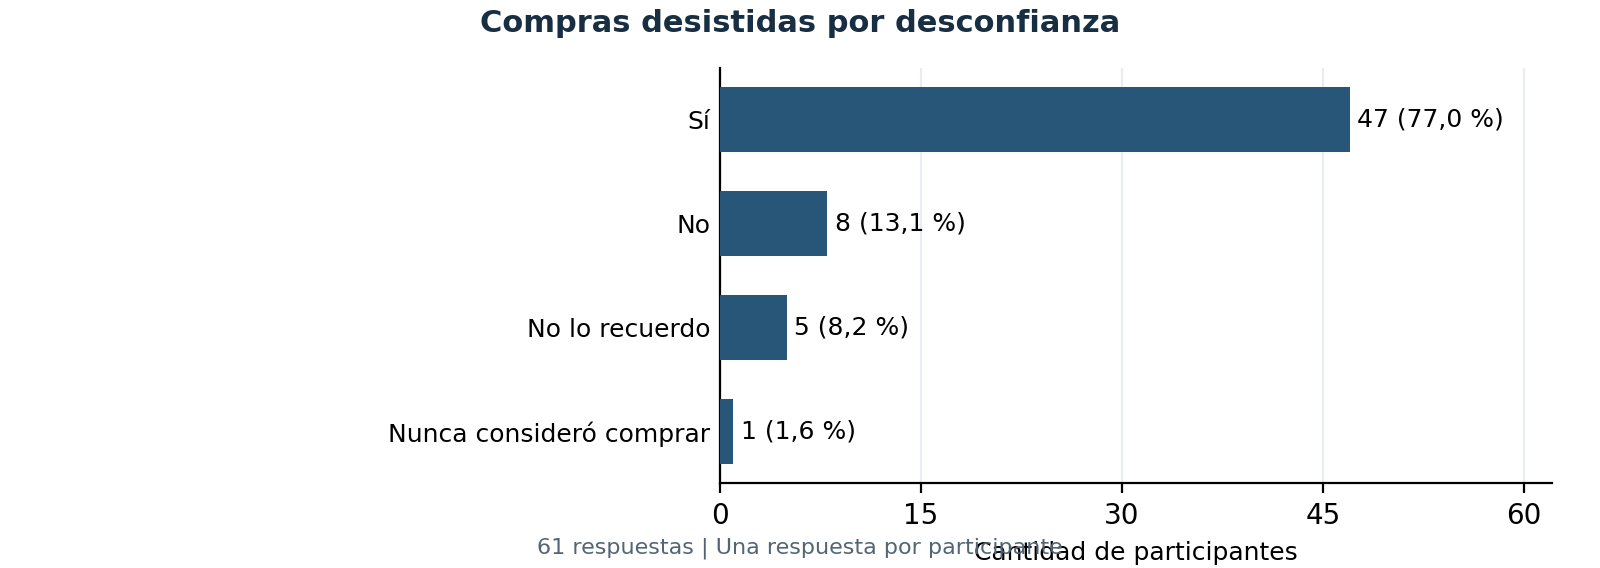
\includegraphics[width=0.94\textwidth,height=0.37\textheight,keepaspectratio]{figuras/marketlens/encuesta/pregunta_05.png}
\caption{Encuestados que desistieron de una compra por desconfianza (n=61).}\label{fig:ml-encuesta-05}
\end{figure}

\begin{figure}[H]
\centering
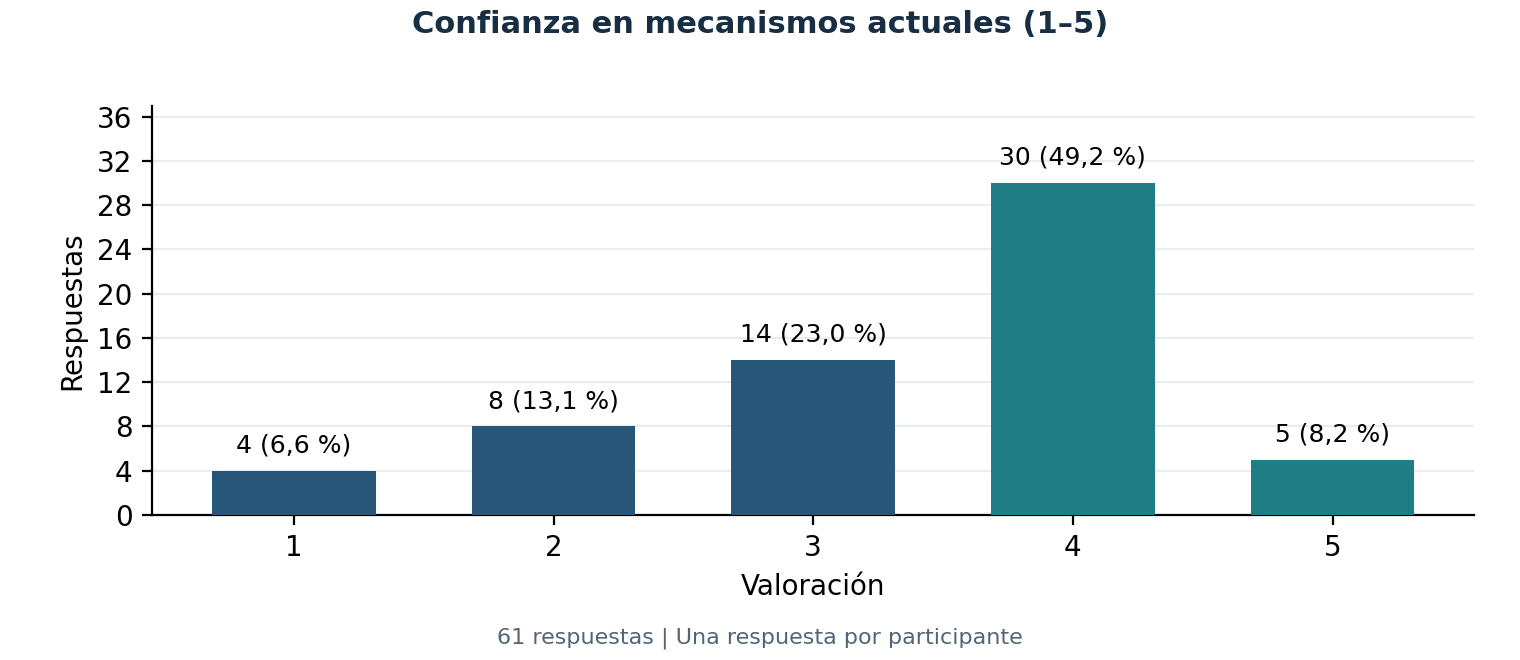
\includegraphics[width=0.94\textwidth,height=0.37\textheight,keepaspectratio]{figuras/marketlens/encuesta/pregunta_06.png}
\caption{Confianza declarada en los mecanismos actuales de seguridad y reputación (n=61).}\label{fig:ml-encuesta-06}
\end{figure}

\begin{figure}[H]
\centering
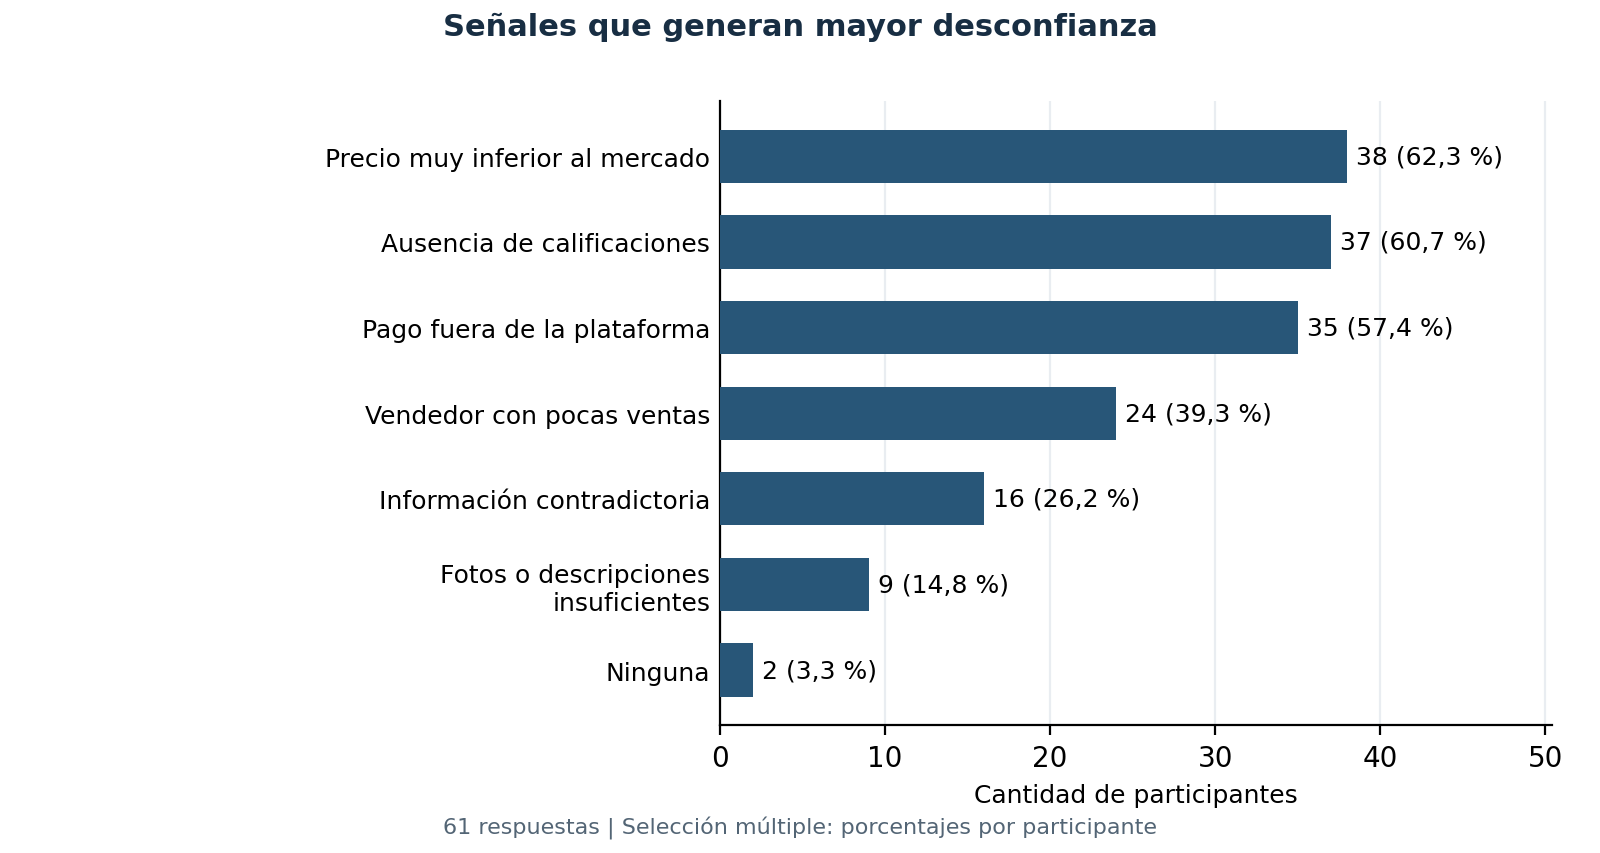
\includegraphics[width=0.94\textwidth,height=0.37\textheight,keepaspectratio]{figuras/marketlens/encuesta/pregunta_07.png}
\caption{Características de publicaciones que generan mayor desconfianza (n=61).}\label{fig:ml-encuesta-07}
\end{figure}

\begin{figure}[H]
\centering
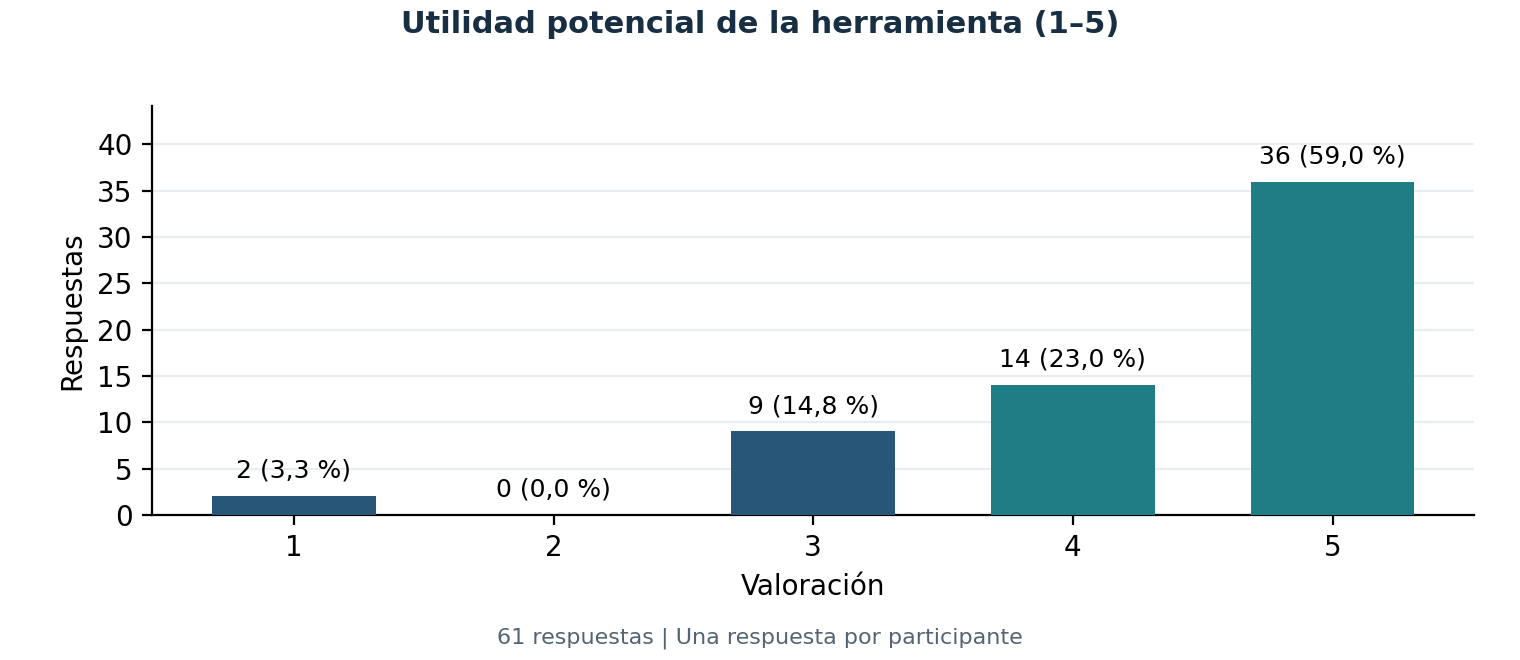
\includegraphics[width=0.94\textwidth,height=0.37\textheight,keepaspectratio]{figuras/marketlens/encuesta/pregunta_08.png}
\caption{Utilidad potencial atribuida a una herramienta de análisis preventivo (n=61).}\label{fig:ml-encuesta-08}
\end{figure}

\begin{figure}[H]
\centering
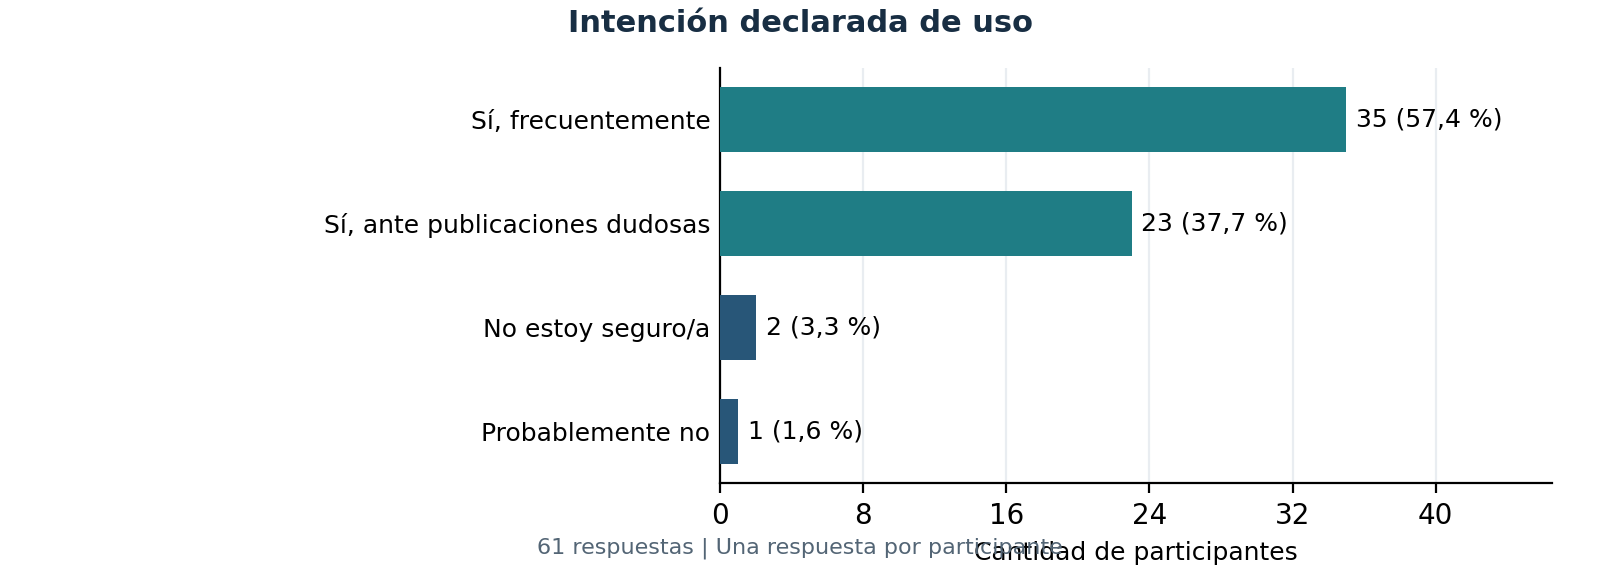
\includegraphics[width=0.94\textwidth,height=0.37\textheight,keepaspectratio]{figuras/marketlens/encuesta/pregunta_09.png}
\caption{Intención declarada de utilización de una herramienta gratuita como la propuesta (n=61).}\label{fig:ml-encuesta-09}
\end{figure}

\begin{figure}[H]
\centering
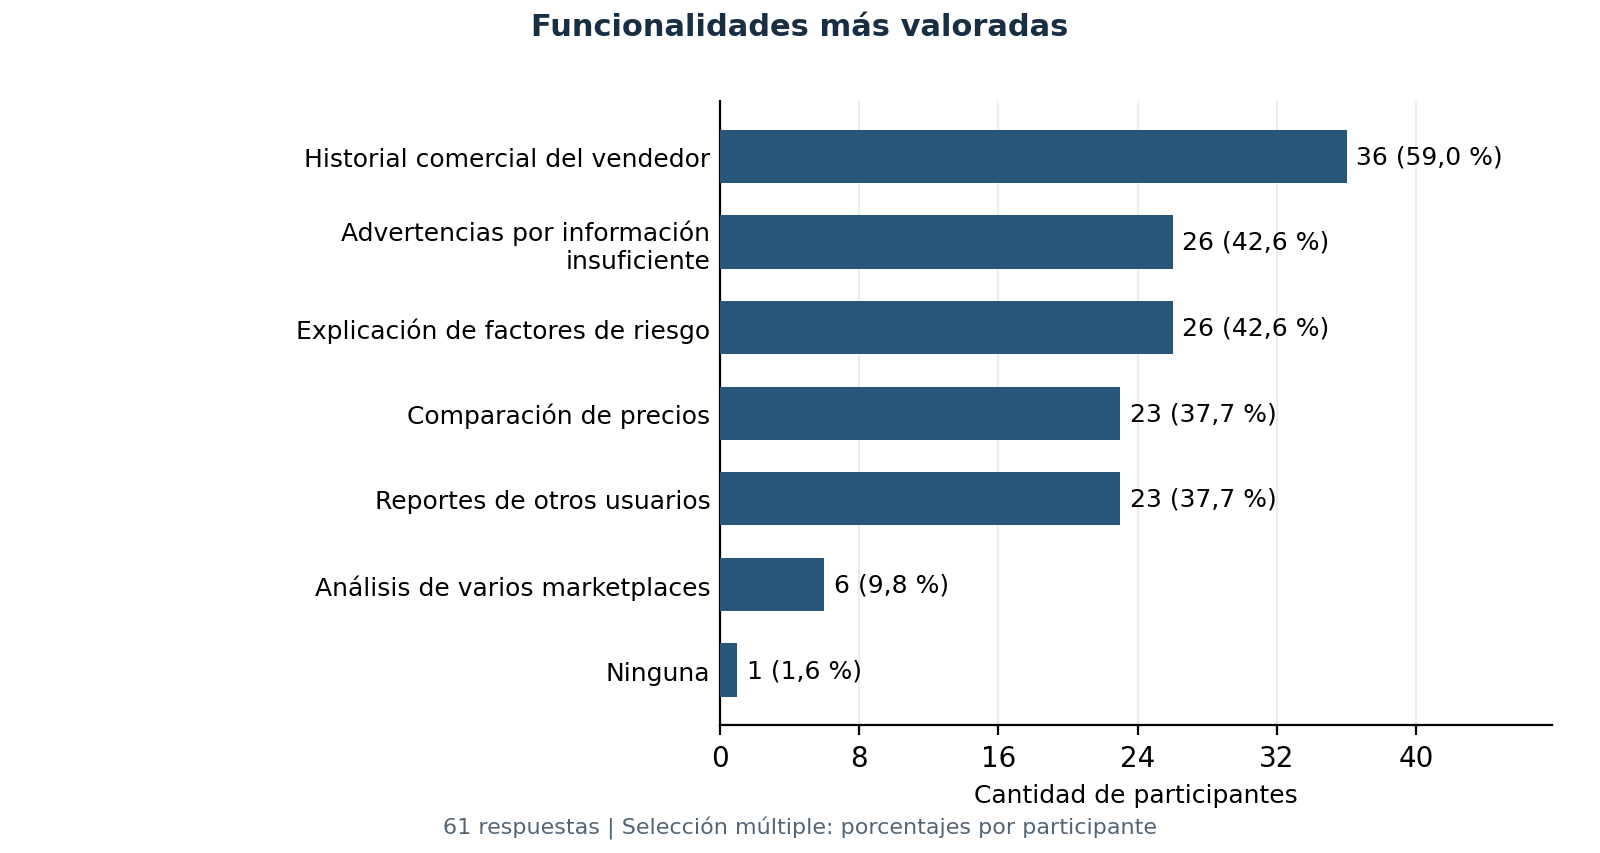
\includegraphics[width=0.94\textwidth,height=0.37\textheight,keepaspectratio]{figuras/marketlens/encuesta/pregunta_10.png}
\caption{Funcionalidades prioritarias para una herramienta de análisis preventivo (n=61).}\label{fig:ml-encuesta-10}
\end{figure}

\begin{figure}[H]
\centering
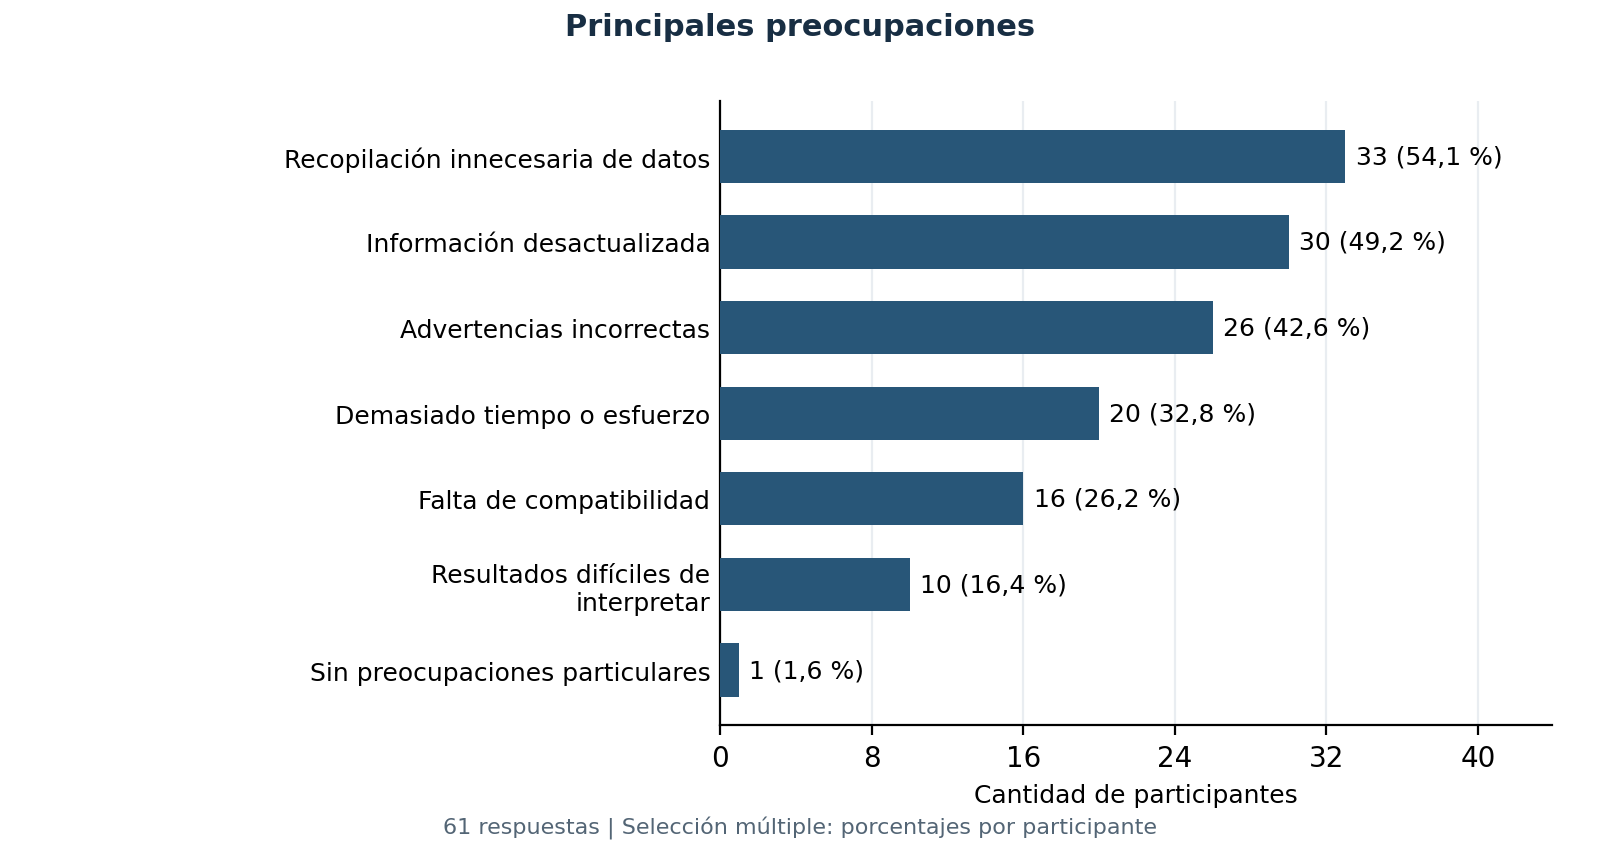
\includegraphics[width=0.94\textwidth,height=0.37\textheight,keepaspectratio]{figuras/marketlens/encuesta/pregunta_11.png}
\caption{Principales preocupaciones respecto del uso de la herramienta (n=61).}\label{fig:ml-encuesta-11}
\end{figure}

